\documentclass[hidelinks]{article}

\usepackage{fancyhdr}
\usepackage{graphicx}
\usepackage{amsmath}
\usepackage{amssymb}
\usepackage{caption}
\usepackage{cancel}
\usepackage{xcolor}
\usepackage{csvsimple}
\usepackage{siunitx}
\usepackage{multicol}
\usepackage{hyperref}
\usepackage{makecell}
\usepackage{listings}
\usepackage[titletoc]{appendix}
\usepackage[margin=1in]{geometry}
\usepackage[style=ieee,backend=biber]{biblatex}
\usepackage[debug, toc, section=section, acronym, symbols]{glossaries} % Glossaries package

\pagestyle{fancy}
\graphicspath{{./img/}}

\begin{document}
	\begin{titlepage}
		\begin{center}
			\vspace{1cm}
			{\LARGE\textbf{Active Band-Pass Filter Project}}
			
			\vspace{1.5cm}
			\textbf{\large Ghassan Arnouk}\\
			
			\vspace{1cm}
			\large ELEC 3509B\\
			\large Summer 2020\\
			\large Lab 4 Report\\
			
			
			\vspace{2cm}
			\textbf{Instructor:} Qi-Jun Zhang\\
			
			
			\vspace{1cm}
			\textbf{Lab Period:} B1\\
			
			\vspace{0.1cm}
			\textbf{Day 1 Preformed:} 2020/08/05
			
			\vspace{0.1cm}
			\textbf{Day 2 Preformed:} 2020/08/06
			
			\vspace{1cm}
			\textbf{Date Submitted:} 2020/08/13\\			
		\end{center}
	\end{titlepage}
	
	\lhead{Ghassan Arnouk (B1)}
	\rhead{Active Band-Pass Filter Project}
	\pagebreak
	
	\tableofcontents
	\pagebreak
	
	\listoftables
	\pagebreak
	
	\listoffigures
	\pagebreak
	
	\section{Introduction}
	Electronic filters are a form of electrical circuits which behaves as a signal processing filter.
	Electronic filters allow wanted components of the applied signal to pass through at certain frequencies, and attenuate unwanted signal components at specific frequencies. 
	Radio communication is an excellent example of the utilization of electronic filters. 
	\subsection{Purpose}
	The purpose of this laboratory is to construct a filter from standardized filter blocks and to provide the junior analog designer an experience with second-order filter circuits as well as the Chebyshev filter response in the context of a design problem [1].
	\subsection{Experiment Overview}
	In day 1, the design calculations of a filter were presented. 
	The design was verified through simulation.
	Data were obtained when performing the simulation.
	Then, useful parameters were measured and compared to the prelab calculated values.\\\\
	In day 2, the design calculations of another filter were presented using industry standard values. 
	The design was verified through simulation.
	Data were obtained when performing the simulation.
	Then, useful parameters were measured and compared to the parameters of the filter when using calculated design values.
	\pagebreak
	\section{Chebyshev Filter Design Project}
	\subsection{Design Requirements}
	The filter to be designed is a fourth order Chebyshev filter.
	This filter is constructed by combining two second order Tow Thomas Biquad filters together.\\
	The Chebyshev filter was designed to satisfy the following requirements:
	\begin{enumerate}
		\item Band-pass action
		\item Chebyshev response
		\item \SI{3}{\decibel} passband ripple
		\item Fourth-order roll-off
		\item Lower cutoff frequency and upper cutoff frequency as calculated below
		\item Target passband gain = +\SI{0.0}{\decibel} to \SI{-3.0}{\decibel}
		\item $\pm$8\% error allowed in $f_{\SI{-3.0}{\decibel}}$
		\item $\pm$\SI{1.0}{\decibel} error allowed in passband gain
		\item Supply voltages to be $\pm$\SI{15}{\volt}
		\item Op-Amps to be type \textbf{TL082} (No more than 6 Op-Amps total)
		\item Output voltage swing $>\pm$\SI{10}{\volt}
	\end{enumerate}
	\subsubsection{Overall Electronic Filter Circuit}
	\subsubsection*{Lower and Upper Cutoff Frequencies, ($f_{\SI{-3}{\decibel}\hspace{1mm} lower}$, $f_{\SI{-3}{\decibel}\hspace{1mm} lower}$):}
	\begin{align*}
		X = 101078550
	\end{align*}
	\begin{align*}
		A = X\ mod\ 1031 = 341\\
		B = X\ mod\ 1033 = 533
	\end{align*}
	\begin{align}
		f_{\SI{-3}{\decibel}\hspace{1mm} lower} &= \frac{A^{5}}{5.534 * 10^{9}} - \frac{A^{4}}{2.11 * 10^{6}} + \frac{A^{3}}{2287} - \frac{A^{2}}{6.1} + \SI{20.0}{\ampere} + 750\\
		&= \frac{341^{5}}{5.534 * 10^{9}} - \frac{341^{4}}{2.11 * 10^{6}} + \frac{341^{3}}{2287} - \frac{341^{2}}{6.1} + \SI{20.0}{\ampere} + 750 \nonumber
	\end{align}
	\begin{align*}
		\therefore f_{\SI{-3}{\decibel}\hspace{1mm} lower} &= \SI{338.64}{\hertz}
	\end{align*}
	\begin{align}
		\delta &= - \frac{B^{2}}{180,000} + \frac{B}{173} + 0.5\\
		&= - \frac{533^{2}}{180,000} + \frac{533}{173} + 0.5 \nonumber\\
		&= 2.0 \nonumber
	\end{align}
	\begin{align}
		f_{\SI{-3}{\decibel}\hspace{1mm} upper} &= f_{\SI{-3}{\decibel}\hspace{1mm} lower} (1 + \delta)\\
		&= (\SI{338.64}{\hertz} )(1+2) \nonumber
	\end{align}
	\begin{align*}
		\therefore f_{\SI{-3}{\decibel}\hspace{1mm} upper} &= \SI{1.0168}{k\hertz}
	\end{align*}
	\pagebreak
	\subsubsection*{Bandwidth:}
	\begin{align}
		%\gls{BW} &= 2\pi (f_{\SI{-3}{\decibel}\hspace{1mm} upper} - f_{\SI{-3}{\decibel}\hspace{1mm} lower})
		BW &= 2\pi (f_{\SI{-3}{\decibel}\hspace{1mm} upper} - f_{\SI{-3}{\decibel}\hspace{1mm} lower})\\
		&= 2\pi (\SI{1.0168}{k\hertz} - \SI{338.64}{\hertz}) \nonumber
	\end{align}
	\begin{align*}
		\therefore BW = \SI{4261}{\radian/ \second}
	\end{align*}
	\subsubsection*{Corner Frequency:}
	\begin{align}
		\omega_o &= 2\pi \sqrt{f_{\SI{-3}{\decibel}\hspace{1mm} upper} * f_{\SI{-3}{\decibel}\hspace{1mm} lower}}\\
		&= 2\pi \sqrt{\SI{1.0168}{k\hertz} - \SI{338.64}{\hertz}} \nonumber
	\end{align}
	\begin{align*}
		\therefore \omega_o = \SI{3687}{\radian/ \second}
	\end{align*}
	\subsubsection*{Quality Factor:}
	\begin{align}
		Q &= \frac{\omega_o}{BW}\\
		&= \frac{\SI{3687}{\radian/ \second}}{\SI{4261}{\radian/ \second}} \nonumber
	\end{align}
	\begin{align*}
		\therefore Q = 0.8653
	\end{align*}
	\subsubsection*{Transfer Function:}
	The general equation for a second order \SI{3}{\decibel} pass-band ripple Chebychev response is as follows:
	\begin{align}
	\label{eqn:tranFun}
		H_2 (S) &= \frac{0.7079 * 0.7079}{S^{2} + 0.6449 S + 0.7079}
	\end{align}
	Using the more generalized equation of the second order \SI{3}{\decibel} pass-band riplle Chebychev response as shown below:
	\begin{align}
		\label{eqn:genFun}
		H_2 (S) = \frac{a^{2}}{S^{2} + b S + c}
	\end{align}
	By comparing Eqs. \ref{eqn:tranFun} and \ref{eqn:genFun}, the variables (a, b, and c) are determined.
	\begin{align}
		\label{eqn:var1}
		a &= 0.7079^2\\
		\label{eqn:var2}
		b &= 0.6449\\
		\label{eqn:var3}
		c &= \sqrt{a} = 0.7079
	\end{align}
	In order to transform the $2^{nd}$ order filter equation to $4^{th}$ order filter equation, we replace:
	\begin{align}
		S &\rightarrow \frac{S^{2} + \omega_o^{2}}{BW S}\\ 
		&= \frac{Q\left[\left(\frac{S}{\omega_o}\right)^{2} + 1\right]}{\left(\frac{S}{\omega_o}\right)}\nonumber\\	
		S &\rightarrow \frac{QS}{\omega_o} + \frac{Q\omega_o}{S} \label{eqn:s}
	\end{align}
	By substiuting Eq. \ref{eqn:s} into Eq. \ref{eqn:genFun}, the $4^{th}$ order filter equation is as follows:
	\begin{align}
	\label{eqn:fourFilter}
		H_4 (S) = \frac{a BW^{2} S^{2}}{S^{4} + b BW^{2} S^{3} + (2\omega_o^{2} + c BW^{2}) S^{2} + b BW^{2} \omega_o^{2} S + \omega_o^{4}}
	\end{align}
	By substiuting Eqs. \ref{eqn:var1}, \ref{eqn:var2}, \ref{eqn:var3} into Eq. \ref{eqn:fourFilter}, we get the following transfer function for the \textbf{\textcolor{green}{overall electronic filter circuit}}:
	\begin{align}
		\label{eqn:fourFilterNum}
		H_4 (S) = \frac{(9.0991 * 10^{6}) S^{2}}{S^{4} + (2780) S^{3} + (4.0042 * 10^{7}) S^{2} + (3.7357 * 10^{10}) S + (1.8480 * 10^{4})}
	\end{align}
	\subsubsection*{Gain}
	Using Fig. \ref{f:overallResponse}, the total gain of the filter circuit is:
	\begin{align*}
		\therefore A_v = \SI{-0.0259}{\decibel}
	\end{align*}
    Using the coefficients of the $4^{th}$ order transfer function, two $2^{nd}$ order transfer functions are obatined.\\
	Splitting Eq. \ref{eqn:fourFilterNum} into two second order transfer functions gives the following:
	\begin{align}
	\label{eqn:4to2}
		H_4 (S) = \frac{(3016.5) S}{S^{2} + (1.9437 * 10^{3}) S + (3.2854 * 10 ^{7})} * \frac{(3016.5) S}{S^{2} + (804.2771) S + (5.6249 * 10 ^{6})}
	\end{align}
	Using Eq. \ref{eqn:4to2}, the transfer functions for the two stages are shown below:
	\begin{align}
		\label{eqn:fun2}
		H_A (S) = \frac{(3016.5) S}{S^{2} + (1.9437 * 10^{3}) S + (3.2854 * 10 ^{7})}\\
		\label{eqn:fun1}
		H_B (S) = \frac{(3016.5) S}{S^{2} + (804.2771) S + (5.6249 * 10 ^{6})}
	\end{align}
	Figure \ref{f:ttf} shows Tow-Thomas second order filter with feedforward which is the circuit used to implement the transfer functions shown in Eqs. \ref{eqn:fun2} and \ref{eqn:fun1}.
	\begin{figure}[htbp]
		\centering
		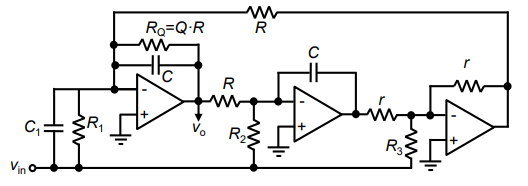
\includegraphics[width=0.7\textheight]{ttCircuit.png}
		\captionof{figure}{Tow-Thomas (with Feedforward) Second Order Filter [1]}
		\label{f:ttf}
	\end{figure}

	\noindent The general form of the transfer function of the circuit shown in Figure \ref{f:ttf} is shown below:
	\begin{align}
		\label{eqn:ttf}
		H(S) &= \frac{S^{2} \left(\frac{C_1}{C}\right) + S \frac{1}{C}\left(\frac{1}{R_1} - \frac{r}{R R_3}\right) + \frac{1}{C^{2} R R_2}}
		{S^{2} + S \frac{\omega_o}{Q} + \left(\frac{1}{RC}\right)^{2}}
	\end{align}
	This filter can realize different filter types. $C, r$ can be fixed arbitrarily. Since a bandpass filter is desired, $C_1 = 0$, $R_2 = \infty$.\\
	Therefore, Eq. \ref{eqn:ttf} can be simplified and written as follows:
	\begin{align}
		\label{eqn:ttfSimplified}
		H(S) &= \frac{S \frac{1}{C}\left(\frac{1}{R_1} - \frac{r}{R R_3}\right)}
		{S^{2} + S \frac{\omega_o}{Q} + \left(\frac{1}{RC}\right)^{2}}
	\end{align} 
	Eq. \ref{eqn:ttfSimplified} has the following generalized form of a $2^{nd}$ order equation which is used to determine the various parameters and characteristics for Eqs. \ref{eqn:fun2} and \ref{eqn:fun1}.
	\begin{align}
		\label{eqn:param}
		H(S) = \frac{a S}{S^{2} + b S+ c}
	\end{align}
	The theoretical response plot of the overall filter circuit is shown in Fig. \ref{f:overallResponse}.
	\begin{figure}[htbp]
		\centering
		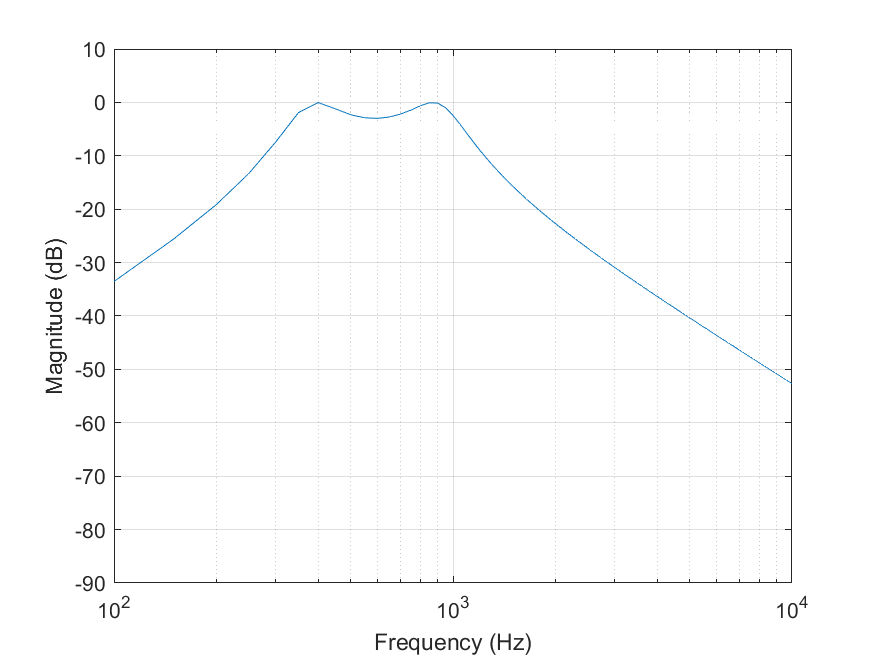
\includegraphics[width=0.6\textheight]{overall_gain.png}
		\captionof{figure}{Theoretical Response Plot of The Overall Filter Circuit}
		\label{f:overallResponse}
	\end{figure}

	\noindent The theoretical response plot of Eqs. \ref{eqn:fun2} and \ref{eqn:fun1} are shown in Fig. \ref{f:aResponse} and Fig. \ref{f:bResponse} respectively.
	\begin{figure}[htbp]
		\centering
		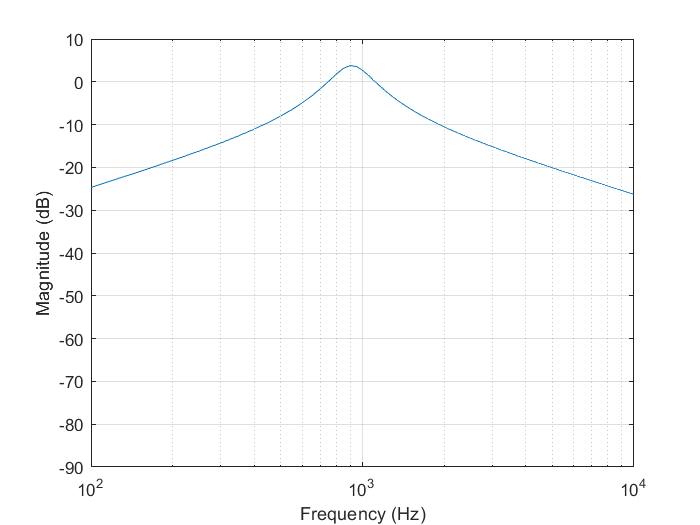
\includegraphics[width=0.6\textheight]{a_gain.png}
		\captionof{figure}{Theoretical Response Plot of The $H_A(S)$ Filter Circuit}
		\label{f:aResponse}
	\end{figure}
	\begin{figure}[htbp]
		\centering
		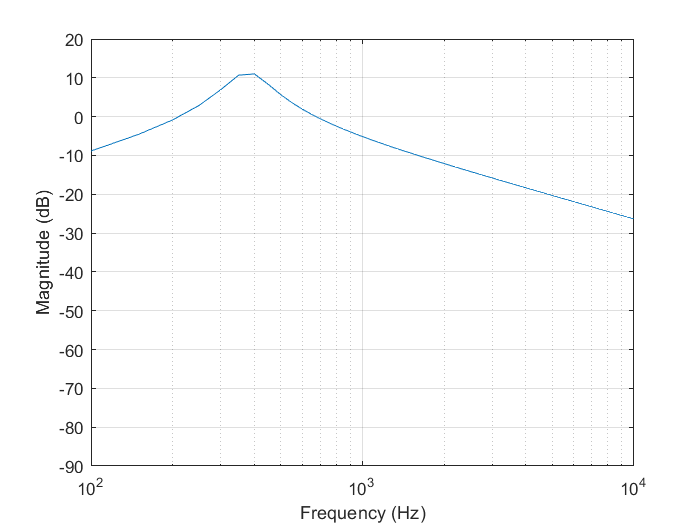
\includegraphics[width=0.6\textheight]{b_gain.png}
		\captionof{figure}{Theoretical Response Plot of The $H_B(S)$ Filter Circuit}
		\label{f:bResponse}
	\end{figure}	
	\pagebreak
	\subsubsection{$H_A(S)$ Parameters}
	By comparing Eqs. \ref{eqn:fun2} and \ref{eqn:param}, the following parameters are determined.
	\subsubsection*{Corner Frequency:}
	\begin{align}
	\omega_{o_A} &= \frac{1}{RC} = \sqrt{c}\\
	&= \sqrt{3.2854 * 10 ^{7}} \nonumber
	\end{align}
	\begin{align*}
	\therefore \omega_{o_A} \approx \SI{5732}{\radian/\second}
	\end{align*}
	\subsubsection*{Bandwidth:}
	\begin{align}
	\label{eqn:bw1}
	BW_A &= \frac{\omega_{o_A}}{Q_A} = b
	\end{align}
	\begin{align*}
	\therefore BW_A = \SI{1943.7}{\radian/\second}
	\end{align*}
	Using Eq. \ref{eqn:bw1}, we get the following:
	\subsubsection*{Quality Factor:}
	\begin{align*}
	\SI{1943.7}{\radian/\second} &= \frac{\SI{5732}{\radian/\second}}{Q_A}\\
	Q_A &= \frac{\SI{5732}{\radian/\second}}{\SI{1943.7}{\radian/\second}}
	\end{align*}
	\begin{align*}
	\therefore Q_A = 2.9488
	\end{align*}
	\subsubsection*{Gain:}
	Using Fig. \ref{f:aResponse}, the gain of this stage is:
	\begin{align*}
	\therefore A_{v_A} = \SI{3.7897}{\decibel}
	\end{align*}
	\subsubsection*{Capacitance Value:}
	$C_A$ is assumed to be \SI{22}{n\farad} as it as a capacitance industry standard value.
	\subsubsection*{Resistance Values:}
	\begin{align}
	R_1 &= \frac{1}{\omega_{o_A} C_A}\\
	&= \frac{1}{(\SI{5732}{\radian/\second}) (\SI{22}{n\farad})} \nonumber
	\end{align}
	\begin{align*}
	\therefore R_{1} = \SI{7.9302}{k\ohm}	
	\end{align*}
	\begin{align}
	R_{q_1} &= R_1* Q_A\\
	&= (\SI{7.9302}{k\ohm}) (2.9488) \nonumber
	\end{align}
	\begin{align*}
	\therefore R_{q_1} = \SI{23.385}{k\ohm}		
	\end{align*}
	
	\pagebreak
	\noindent Assuming $r_A = R_{q_1} = \SI{23.385}{k\ohm}$, for simplicity, we get the following:
	\begin{align}
	R_{31} &= \frac{r_A}{a R_1 C_A}\\
	&= \frac{\SI{23.385}{k\ohm}}{(3016.5) (\SI{7.9302}{k\ohm}) (\SI{22}{n\farad})} \nonumber
	\end{align}
	\begin{align*}
	\therefore R_{31} &= \SI{44.435}{k\ohm}
	\end{align*}	
	
	
	
	\pagebreak
	\subsubsection{$H_B(S)$ Parameters}
	By comparing Eqs. \ref{eqn:fun1} and \ref{eqn:param}, the following parameters are determined.
	\subsubsection*{Corner Frequency:}
	\begin{align}
		\omega_{o_B} &= \frac{1}{RC} = \sqrt{c}\\
		&= \sqrt{5.6249 * 10 ^{6}} \nonumber
	\end{align}
	\begin{align*}
		\therefore \omega_{o_B} \approx \SI{2372}{\radian/\second}
	\end{align*}
	\subsubsection*{Bandwidth:}
	\begin{align}
		\label{eqn:bw}
		BW_B &= \frac{\omega_{o_B}}{Q_B} = b
	\end{align}
	\begin{align*}
		\therefore BW_B = \SI{804.2771}{\radian/\second}
	\end{align*}
	Using Eq. \ref{eqn:bw}, we get the following:
	\subsubsection*{Quality Factor:}
	\begin{align*}
		\SI{804.2771}{\radian/\second} &= \frac{\SI{2372}{\radian/\second}}{Q_B}\\
		Q_B &= \frac{\SI{2372}{\radian/\second}}{\SI{804.2771}{\radian/\second}}
	\end{align*}
	\begin{align*}
		\therefore Q_B = 2.9488
	\end{align*}
	\subsubsection*{Gain:}
	Using Fig. \ref{f:bResponse}, the gain of this stage is:
	\begin{align*}
		\therefore A_{v_B} = \SI{11}{\decibel}
	\end{align*}
	\subsubsection*{Capacitance Value:}
	$C_B$ is assumed to be \SI{33}{n\farad} as it as a capacitance industry standard value.
	\subsubsection*{Resistance Values:}
	\begin{align}
		R_2 &= \frac{1}{\omega_{o_B} C_B}\\
		&= \frac{1}{(\SI{2372}{\radian/\second}) (\SI{33}{n\farad})} \nonumber
	\end{align}
	\begin{align*}
		\therefore R_{2} = \SI{12.777}{k\ohm}	
	\end{align*}
	\begin{align}
		R_{q_2} &= R_2* Q_B\\
		&= (\SI{12.777}{k\ohm}) (2.9488) \nonumber
	\end{align}
	\begin{align*}
		\therefore R_{q_2} = \SI{37.677}{k\ohm}		
	\end{align*}
	
	\pagebreak
	\noindent Assuming $r_B = R_{q_2} = \SI{37.677}{k\ohm}$, for simplicity, we get the following:
	\begin{align}
		R_{32} &= \frac{r_B}{a R_2 C_B}\\
		&= \frac{\SI{37.677}{k\ohm}}{(3016.5) (\SI{12.777}{k\ohm}) (\SI{33}{n\farad})} \nonumber
	\end{align}
	\begin{align*}
		\therefore R_{32} &= \SI{29.624}{k\ohm}
	\end{align*}
	
	\pagebreak
	\noindent The overall filter circuit with the theoretical (calculated) components values is shown in Fig. \ref{f:overallCirTheo}.
	\begin{figure}[htbp]
		\centering
		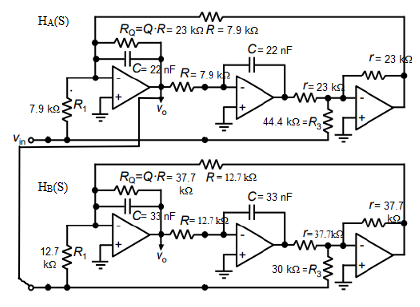
\includegraphics[width=0.6\textheight]{overallfun.png}
		\captionof{figure}{The Overall Filter Circuit With The Theoretical Components Values [1]}
		\label{f:overallCirTheo}
	\end{figure}

	\pagebreak	
	\noindent The circuit that represent each of Eqs. \ref{eqn:fun2} and \ref{eqn:fun1} are shown in Fig. \ref{f:afun} and Fig. \ref{f:bfun} respectively.
	\begin{figure}[htbp]
		\centering
		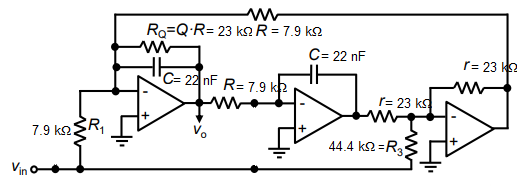
\includegraphics[width=0.6\textheight]{afun.png}
		\captionof{figure}{The $H_A(S)$ Filter Circuit With The Theoretical Components Values [1]}
		\label{f:afun}
	\end{figure}
	\begin{figure}[htbp]
		\centering
		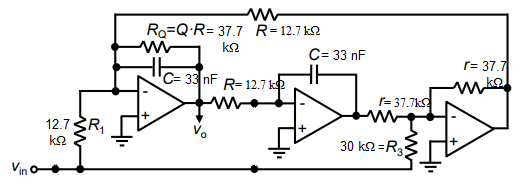
\includegraphics[width=0.6\textheight]{bfun.png}
		\captionof{figure}{The $H_B(S)$ Filter Circuit With The Theoretical Components Values [1]}
		\label{f:bfun}
	\end{figure}
	
	\pagebreak	
	\subsection{Simulation}
	\subsubsection{Simulated Filter Circuit}
	Fig. \ref{f:circuit1} illustrates the overall filter circuit used in this part of the experiment.
	\begin{figure}[htbp]
		\centering
		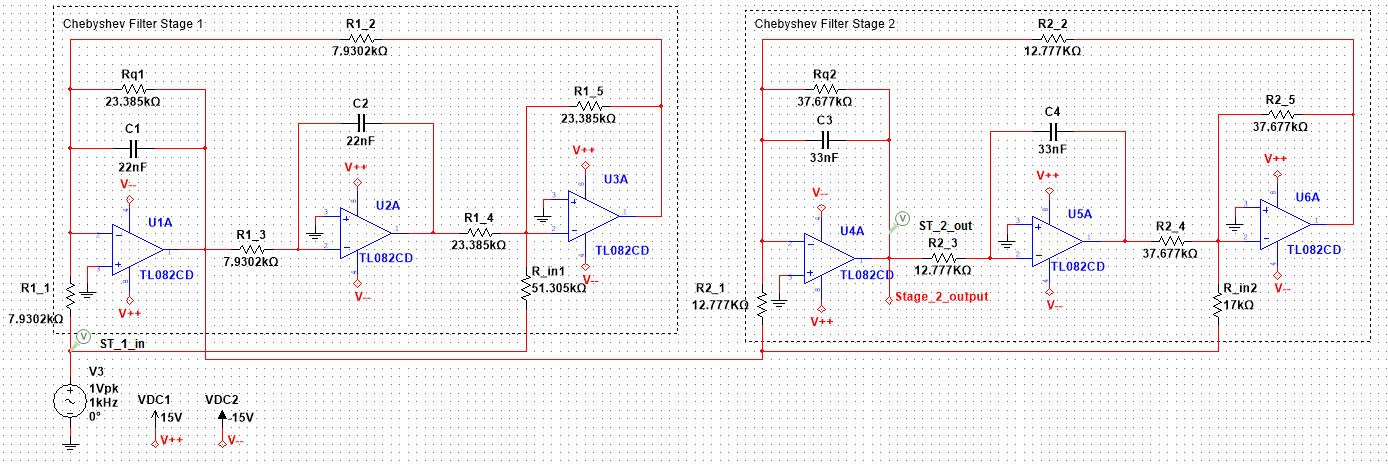
\includegraphics[width=0.65\textheight]{circuit1.png}
		\captionof{figure}{The Simulated Overall Filter Circuit With Theoretical Components Values}
		\label{f:circuit1}
	\end{figure}

	\noindent Fig. \ref{f:settings} illustrates the AC sweep settings of the overall filter circuit used in this part of the experiment.
		\begin{figure}[htbp]
		\centering
		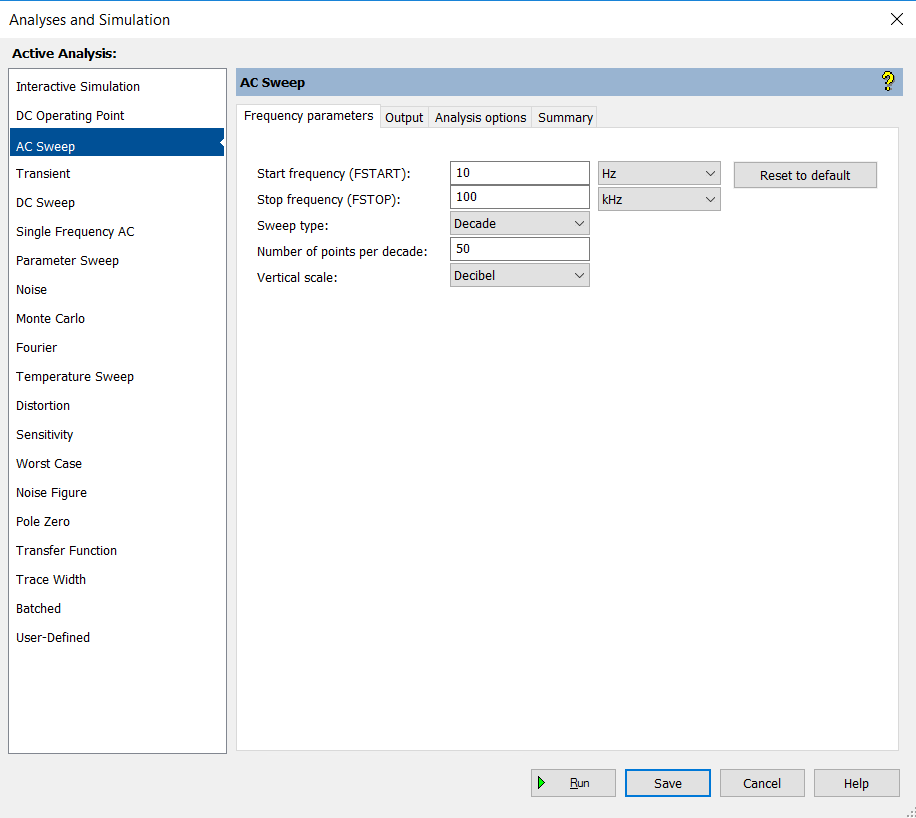
\includegraphics[width=0.5\textheight]{sim_settings.png}
		\captionof{figure}{Overall Filter Circuit AC Sweep Simulation Settings}
		\label{f:settings}
	\end{figure}
	
	\pagebreak
	\noindent Fig. \ref{f:overall_working} shows the simulated response plot of the overall filter circuit.
	\begin{figure}[htbp]
		\centering
		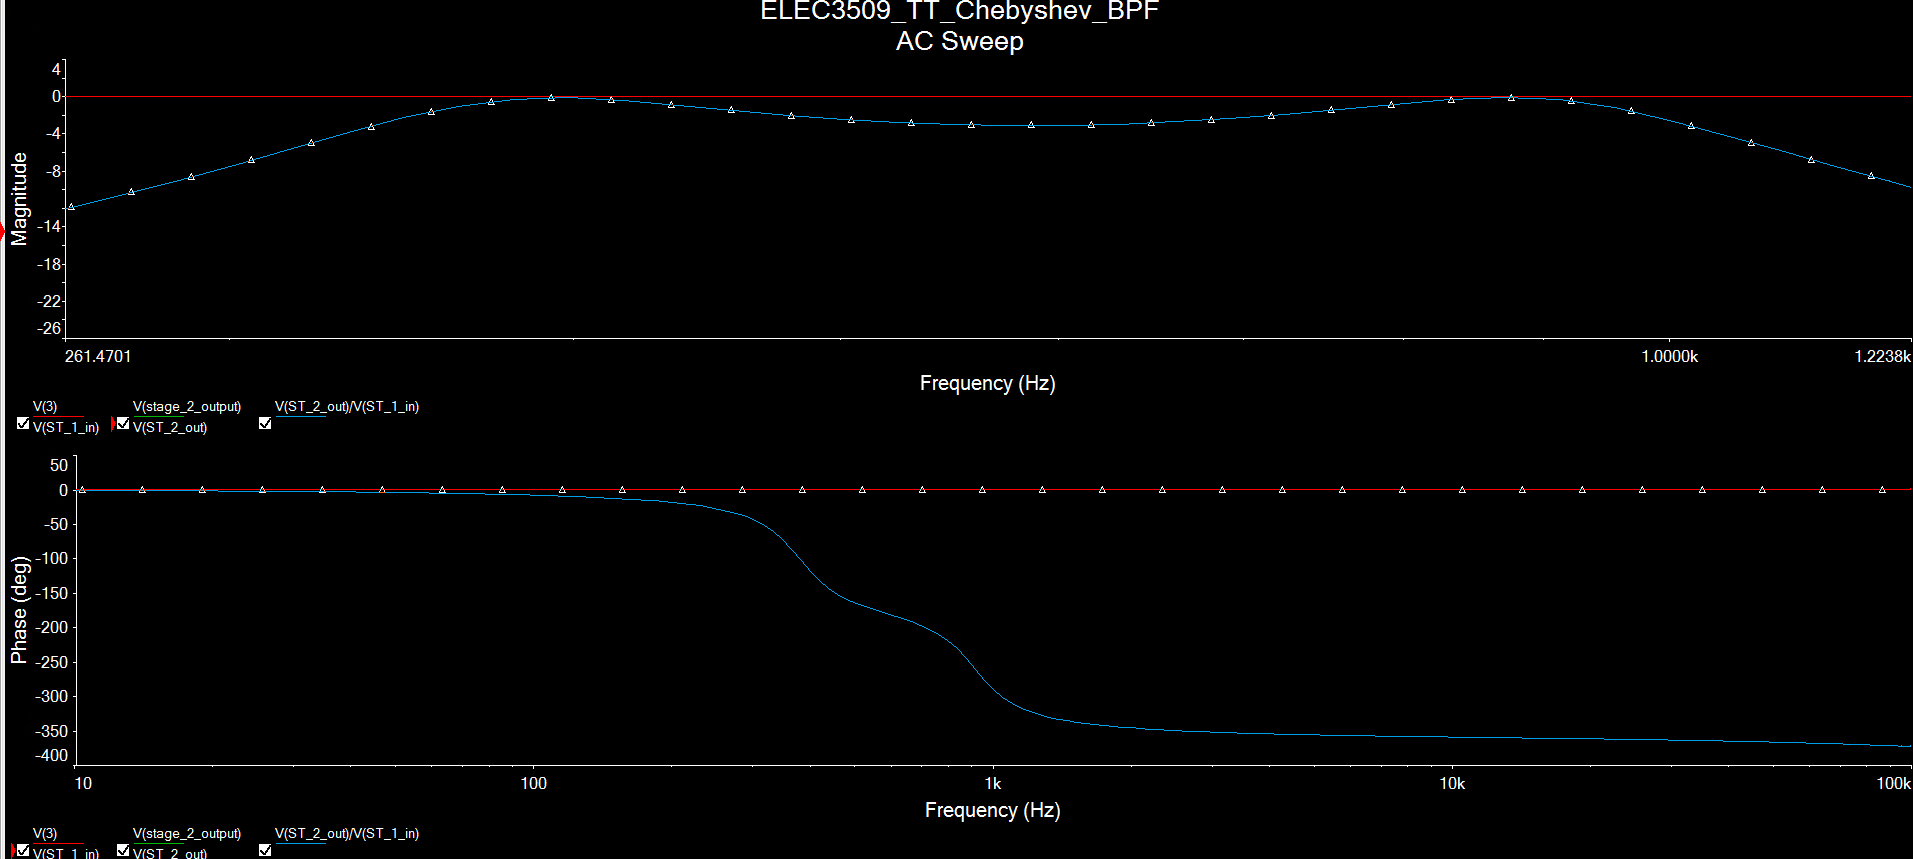
\includegraphics[width=0.7\textheight]{overall_working.png}
		\captionof{figure}{Overall Filter Circuit Simulated Response Plot}
		\label{f:overall_working}
	\end{figure}

	\noindent As shown in Fig. \ref{f:circuit1}, $R_{in_1}$ is increased and set to approximately \SI{51}{k\ohm} while the theoretical value is \SI{44.4}{k\ohm}. 
	Likewise, $R_{in_2}$ is decreased and set to \SI{17}{k\ohm} while the theoretical value is approximately \SI{30}{k\ohm} before performing the simulation.
	These changes in the circuit were made to achieve the desired voltage gain of the overall filter circuit.
	If the theoretical values were used, the voltage gain would be around \SI{-14}{\decibel}. However, the simulated plot shows the desireable gain of approximately \SI{0}{\decibel}.
	Similarly, if the theoretical values of $R_{in_1}$ and $R_{in_2}$, the frequency values would have exceeded $\pm$8\% error which does not satisfy the requirements of this project.
	Fig. \ref{f:overall_working} shows the gain in the simulated response plot which is an exact match of the theoretical response plot as shown in Fig. \ref{f:overallResponse}.\\\\
	Note that the simulated response plot of the individual $2^{nd}$ order filter circuits were done while maintaining the changes done to $R_{in_1}$ and $R_{in_2}$ for the exact same reasons.\\\\
	\textcolor{red}{\textbf{Note:}} Data were presented on the gain plot and are shown in Fig. \ref{f:measured_simulated}.
	
	\pagebreak
	\noindent Fig. \ref{f:circuit2} illustrates each of the individual $2^{nd}$ order filter circuits, $H_A(S)$ and $H_B(S)$ respectively, used in this part of the experiment.
	\begin{figure}[htbp]
		\centering
		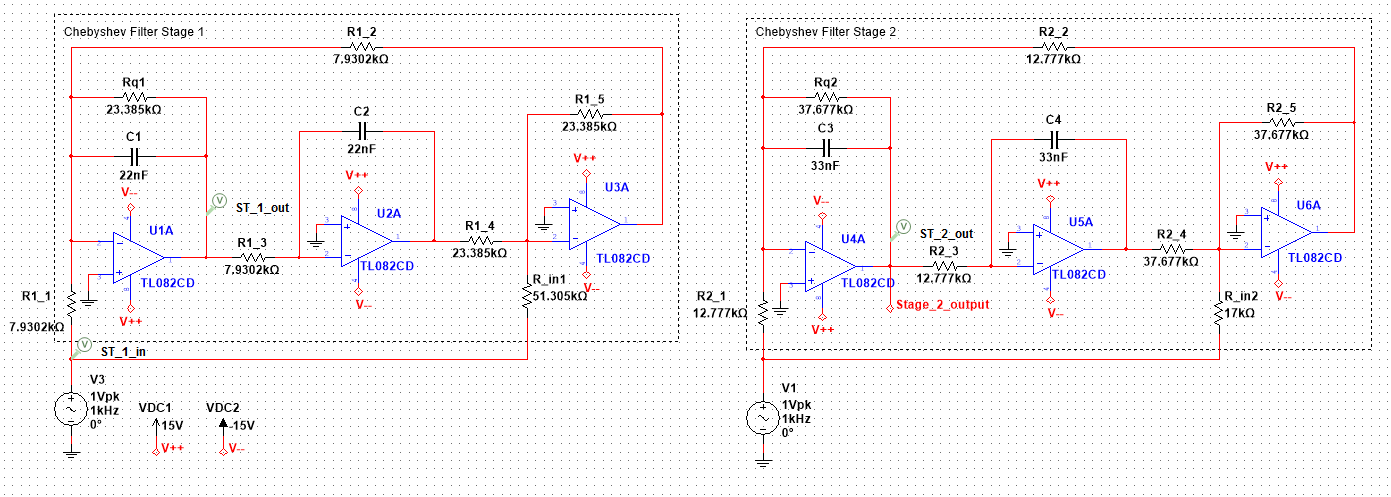
\includegraphics[width=0.65\textheight]{circuit2.png}
		\captionof{figure}{The Simulated Individual Filter Circuits With Theoretical Components Values}
		\label{f:circuit2}
	\end{figure}
	
	\noindent Fig. \ref{f:settings1} illustrates the AC sweep settings of each of the individual $2^{nd}$ order filter circuits, $H_A(S)$ and $H_B(S)$ respectively, used in this part of the experiment.
	\begin{figure}[htbp]
		\centering
		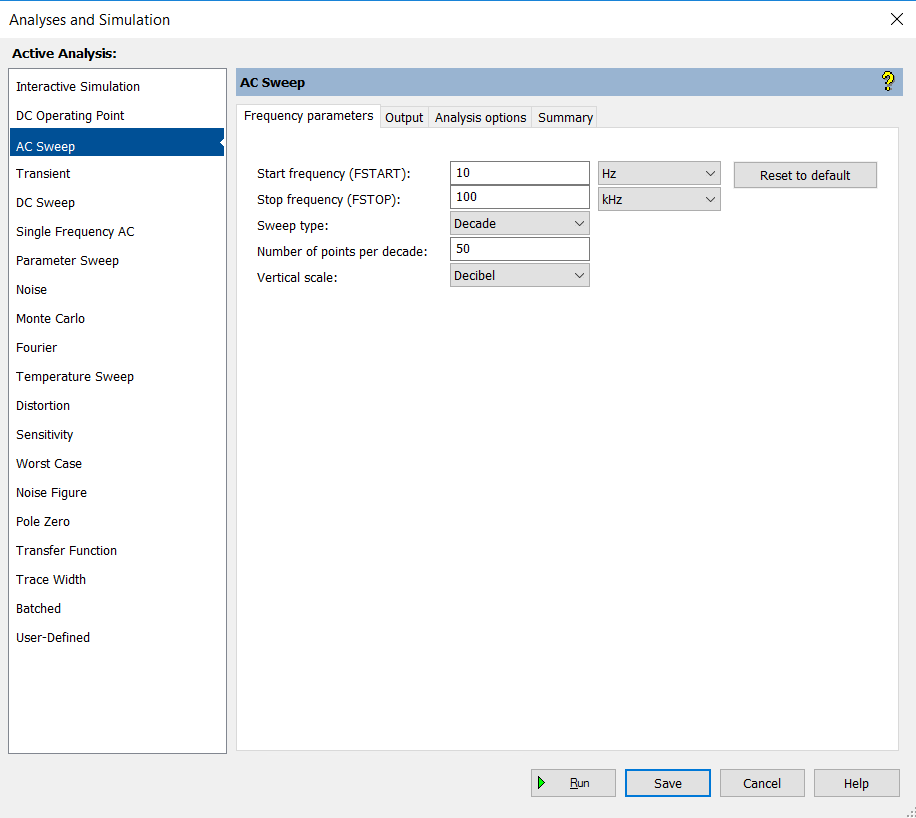
\includegraphics[width=0.65\linewidth]{sim_settings1.png}
		\captionof{figure}{Overall Filter Circuit AC Sweep Simulation Settings}
		\label{f:settings1}
	\end{figure}	
	
	\pagebreak
	\noindent Fig. \ref{f:stageA_gain} and Fig. \ref{f:stageB_gain} show the simulated response plot of the individual $2^{nd}$ order filter circuits of $H_A(S)$ and $H_B(S)$ respectively.
	\begin{figure}[htbp]
		\centering
		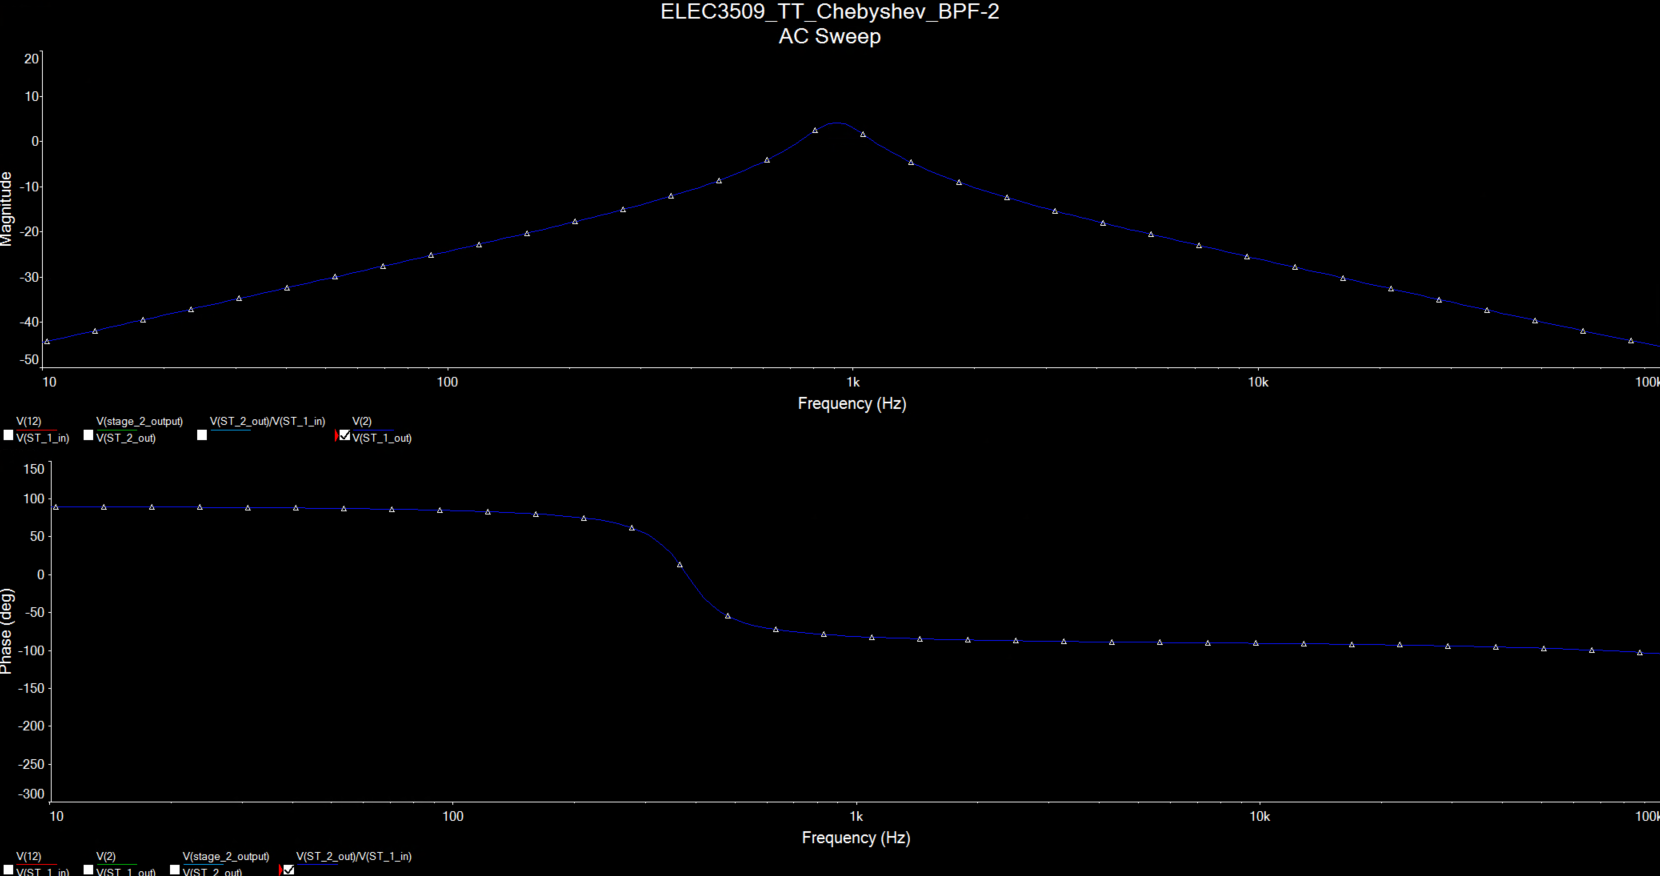
\includegraphics[width=0.6\textheight]{stageA_gain.png}
		\captionof{figure}{Simulated Response Plot of The $H_A(S)$ Filter Circuit}
		\label{f:stageA_gain}
	\end{figure}	
	\begin{figure}[htbp]
		\centering
		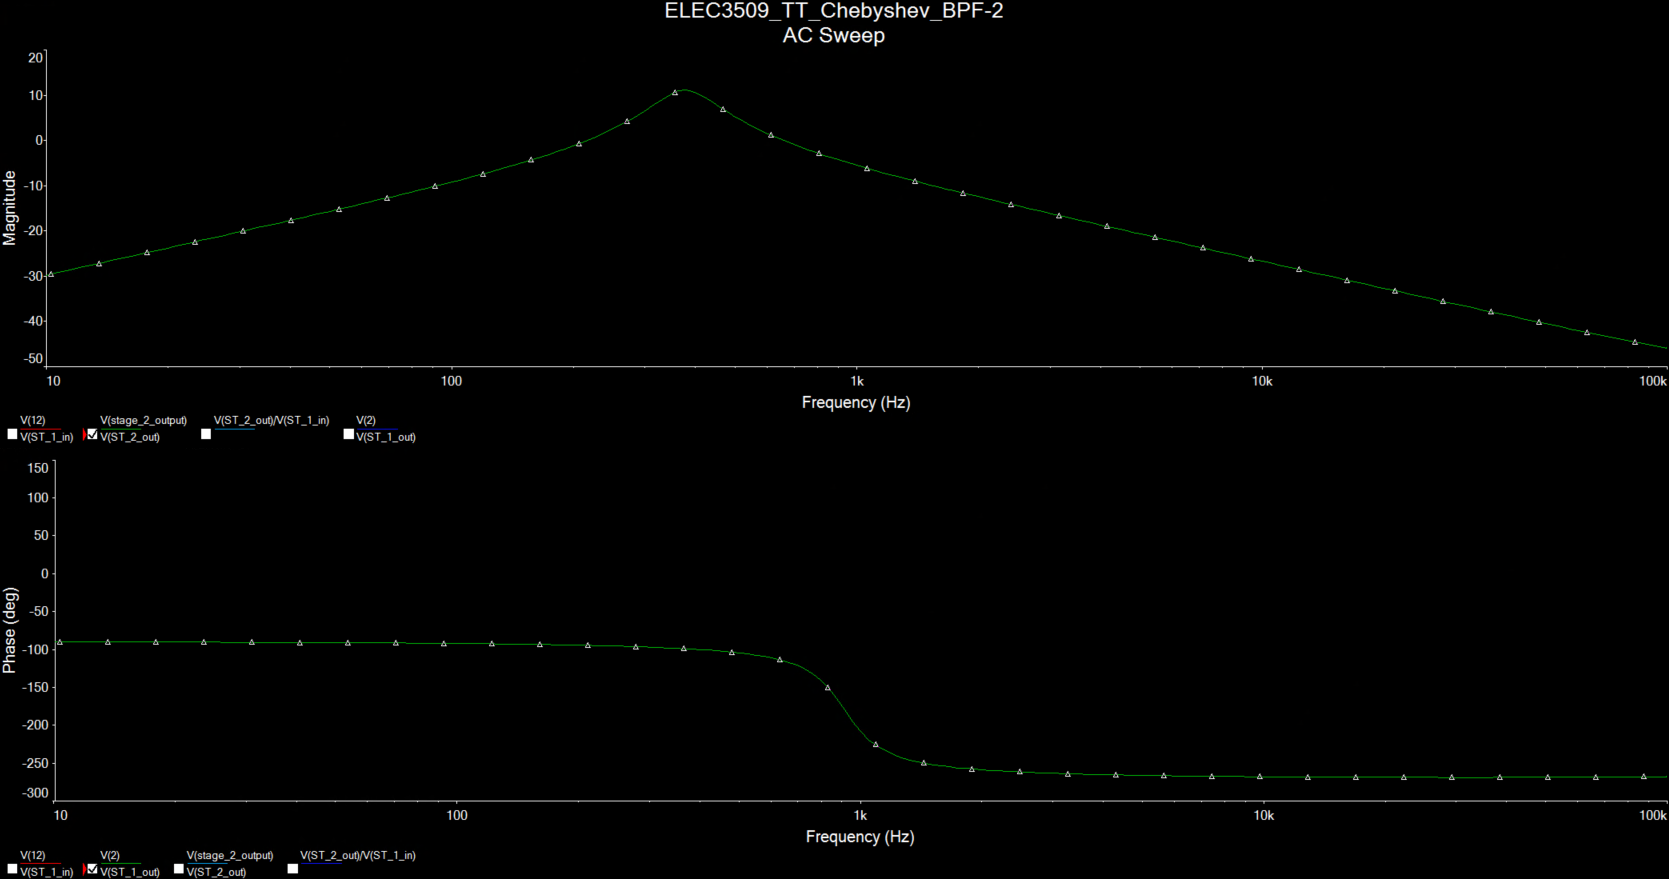
\includegraphics[width=0.6\textheight]{stageB_gain.png}
		\captionof{figure}{Simulated Response Plot of The $H_B(S)$ Filter Circuit}
		\label{f:stageB_gain}
	\end{figure}	

	\noindent In comparison between Fig. \ref{f:stageA_gain} and Fig. \ref{f:aResponse}, the gain in the simulated response plot is an exact match of the theoretical response plot for $H_A(S)$. 
	Likewise, the comparison between Fig. \ref{f:stageB_gain} and Fig. \ref{f:bResponse} shows that the gain in the simulated response plot is an exact match of the theoretical response plot for $H_B(S)$.
	
	\pagebreak
	\subsubsection{Standard Simulated Filter Circuit}	
	Fig. \ref{f:overallStand} illustrates the overall filter circuit with standard values used in this part of the experiment.
	\begin{figure}[htbp]
		\centering
		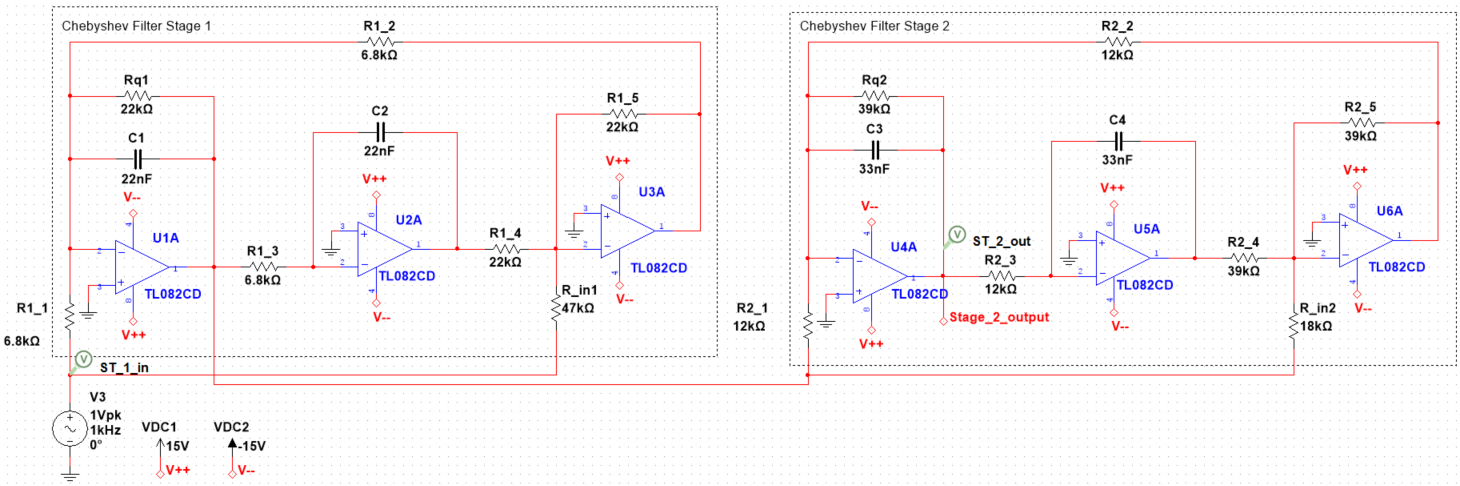
\includegraphics[width=0.7\textheight]{circuit3.png}
		\captionof{figure}{The Simulated Overall Filter Circuit With Standard Components Values}
		\label{f:overallStand}
	\end{figure}

	\noindent Fig. \ref{f:sim_settings2} illustrates the AC sweep settings of the overall filter circuit used in this part of the experiment.
	\begin{figure}[htbp]
		\centering
		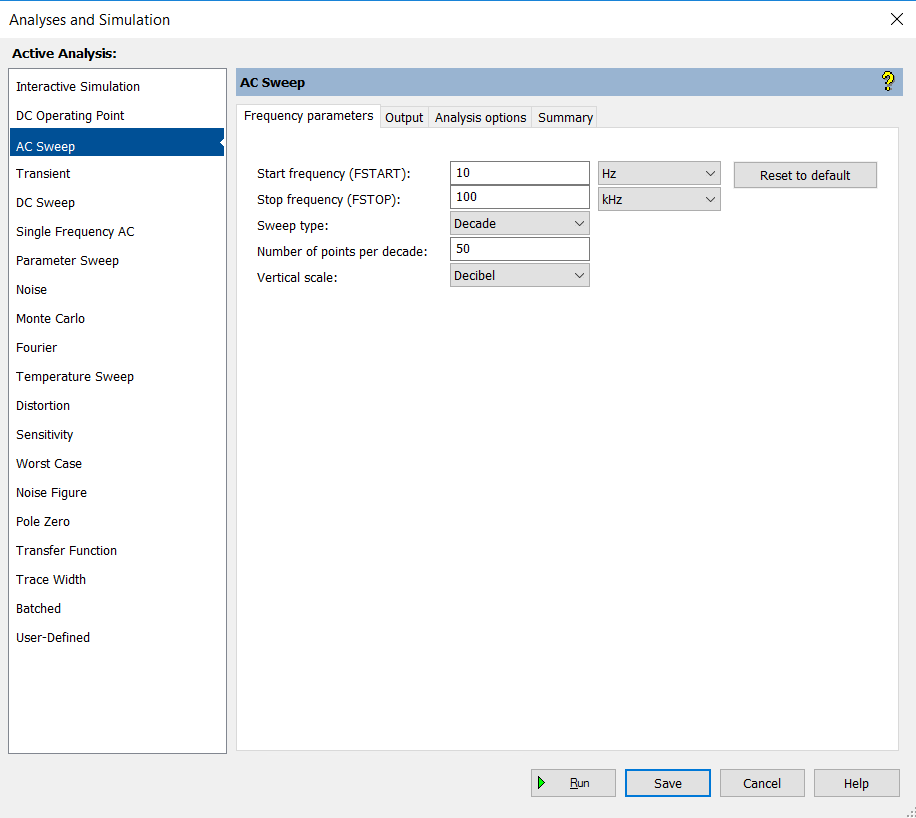
\includegraphics[width=0.65\linewidth]{sim_settings2.png}
		\captionof{figure}{The Simulated Overall Filter Circuit With Standard Components Values}
		\label{f:sim_settings2}
	\end{figure}	

	\pagebreak
	\noindent Fig. \ref{f:sim_overallStand} shows the simulated response plot of the overall filter circuit using standard components values.
	\begin{figure}[htbp]
		\centering
		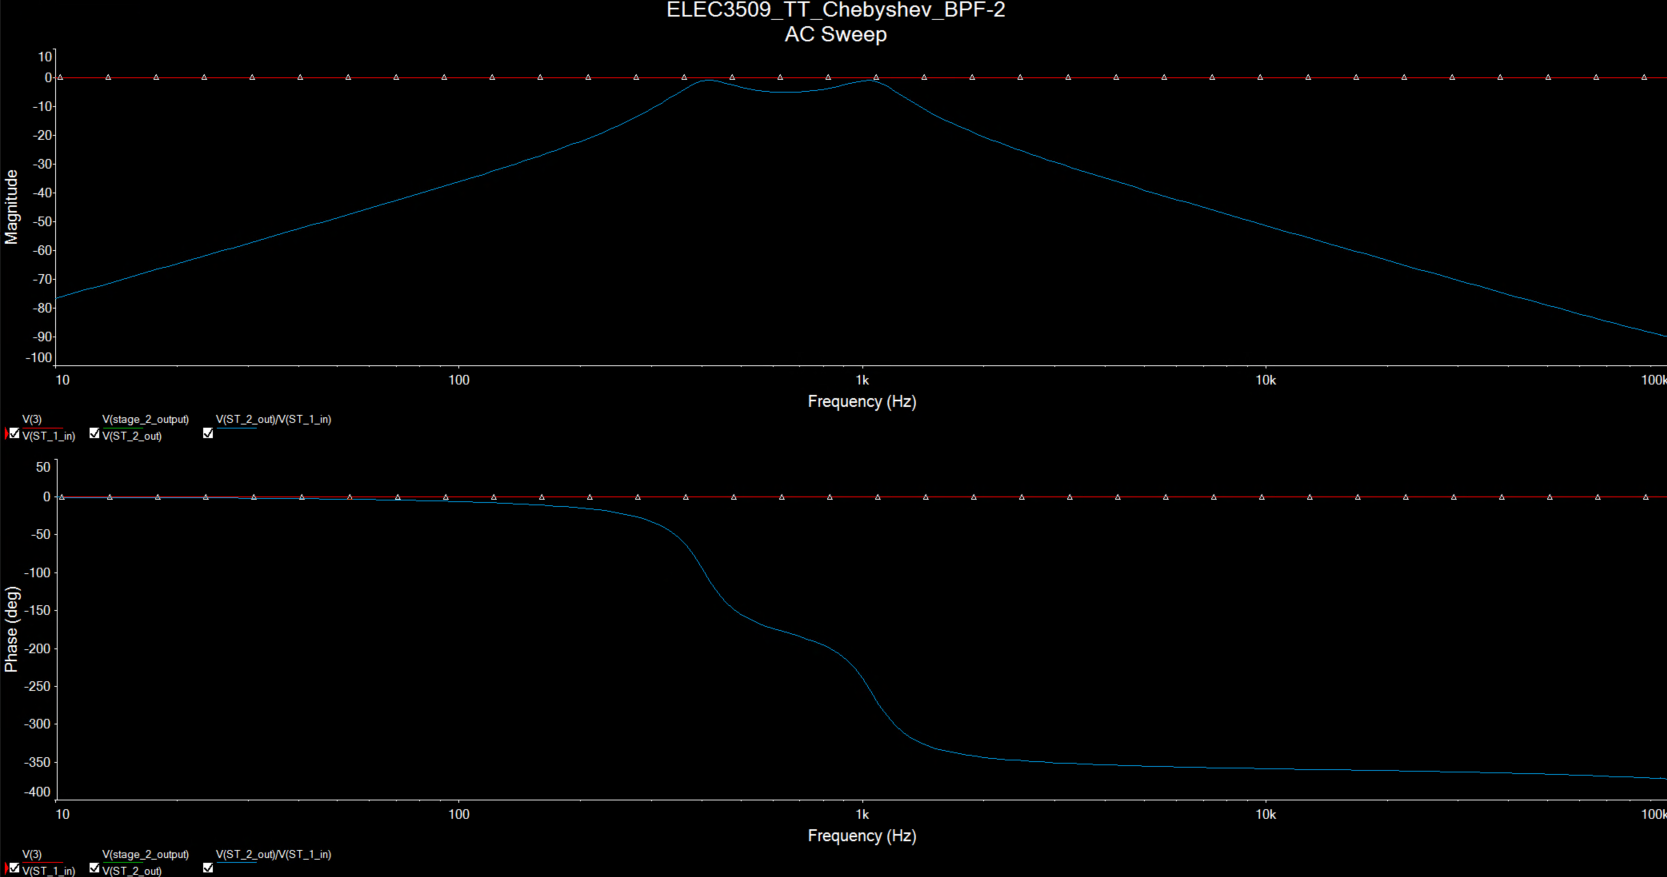
\includegraphics[width=0.7\textheight]{sim_overallStand.png}
		\captionof{figure}{The Simulated Overall Filter Circuit With Standard Components Values}
		\label{f:sim_overallStand}
	\end{figure}	
	
	\noindent As shown in Fig. \ref{f:sim_overallStand}, $R_{in_1}$ is increased and set to a standard value of \SI{47}{k\ohm} while the theoretical value is \SI{44.4}{k\ohm}. 
	Likewise, $R_{in_2}$ is decreased and set to a standard value of \SI{18}{k\ohm} while the theoretical value is approximately \SI{30}{k\ohm} before performing the simulation.
	Also, $R_{11}$, $R_{12}$, and $R_{13}$ are set to a standard value of \SI{6.8}{k\ohm} while the theoretical value is approximately \SI{8}{k\ohm}.
	These changes in the circuit were made to achieve the desired voltage gain of the overall filter circuit.
	The closest standard values to the theoretical values were used, the voltage gain would be around \SI{-10}{\decibel}. However, the simulated plot shows the desireable gain of approximately \SI{0}{\decibel} after performing few changes to components values.
	Similarly, if the theoretical values of $R_{in_1}$, $R_{in_2}$, $R_{11}$, $R_{12}$, and $R_{13}$, the frequency values would have exceeded $\pm$8\% error which does not satisfy the requirements of this project.
	Fig. \ref{f:sim_overallStand} shows the gain in the simulated response plot using standard components values which is fairly a match of the theoretical and simulated response plots as shown in Fig. \ref{f:overall_working} and Fig. \ref{f:overallResponse}.\\\\
	Note that the simulated response plot of the individual $2^{nd}$ order filter circuits using standard components values were done while maintaining the changes done to $R_{in_1}$ and $R_{in_2}$ for the exact same reasons.\\\\
	\textcolor{red}{\textbf{Note:}} Data were presented on the gain plot and are shown in Fig. \ref{f:measured_standSimulated}.
	
	\pagebreak
	\noindent Fig. \ref{f:circuit4} illustrates each of the individual $2^{nd}$ order filter circuits using standard components values, $H_A(S)$ and $H_B(S)$ respectively, used in this part of the experiment.
	\begin{figure}[htbp]
		\centering
		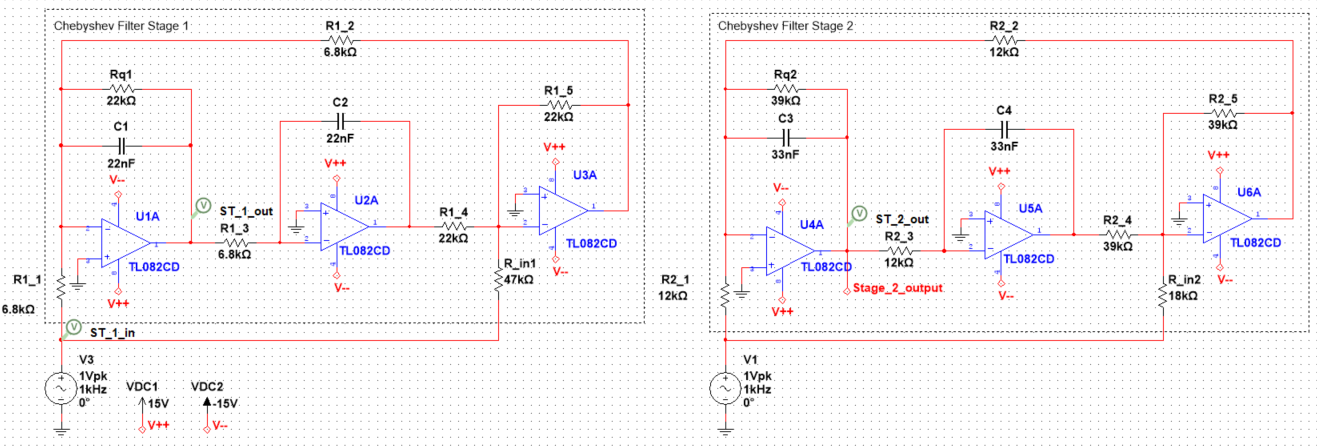
\includegraphics[width=0.65\textheight]{circuit4.png}
		\captionof{figure}{The Simulated Individual Filter Circuits With Standard Components Values}
		\label{f:circuit4}
	\end{figure}
	
	\noindent Fig. \ref{f:sim_settings3} illustrates the AC sweep settings of each of the individual $2^{nd}$ order filter circuits, $H_A(S)$ and $H_B(S)$ respectively, used in this part of the experiment.
	\begin{figure}[htbp]
		\centering
		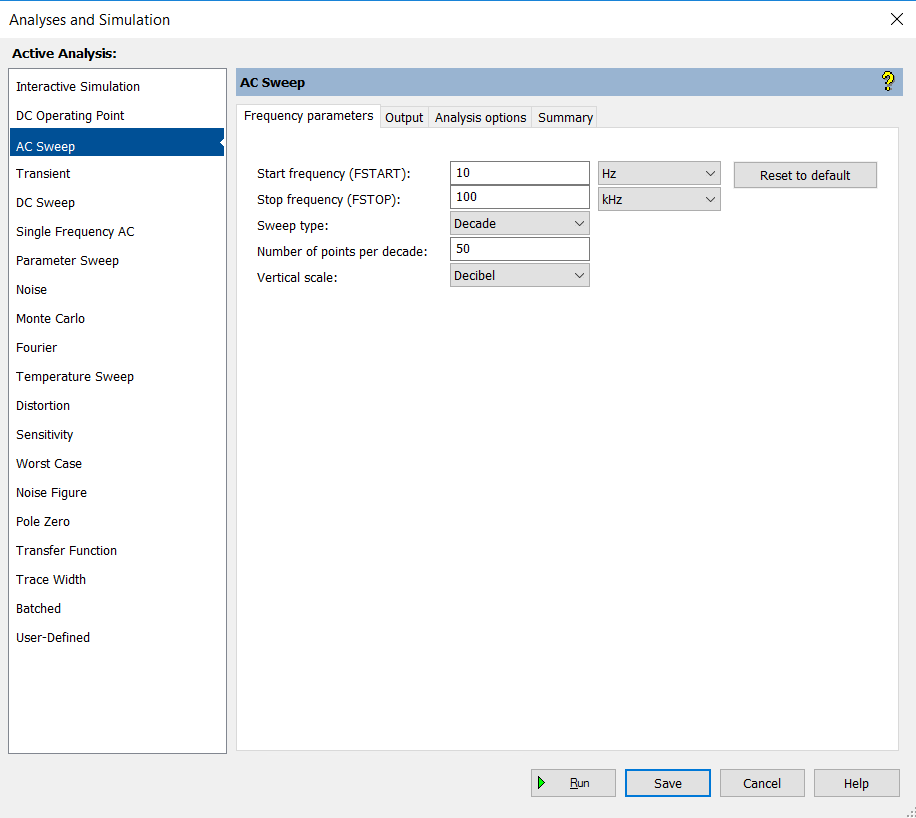
\includegraphics[width=0.65\linewidth]{sim_settings3.png}
		\captionof{figure}{Individual Filter Circuits AC Sweep Simulation Settings}
		\label{f:sim_settings3}
	\end{figure}	
	
	\pagebreak	
	\noindent Fig. \ref{f:stageA_gain_stand} and Fig. \ref{f:stageB_gain_stand} show the simulated response plot of the individual $2^{nd}$ order filter circuits, using standard components values, of $H_A(S)$ and $H_B(S)$ respectively.
	\begin{figure}[htbp]
		\centering
		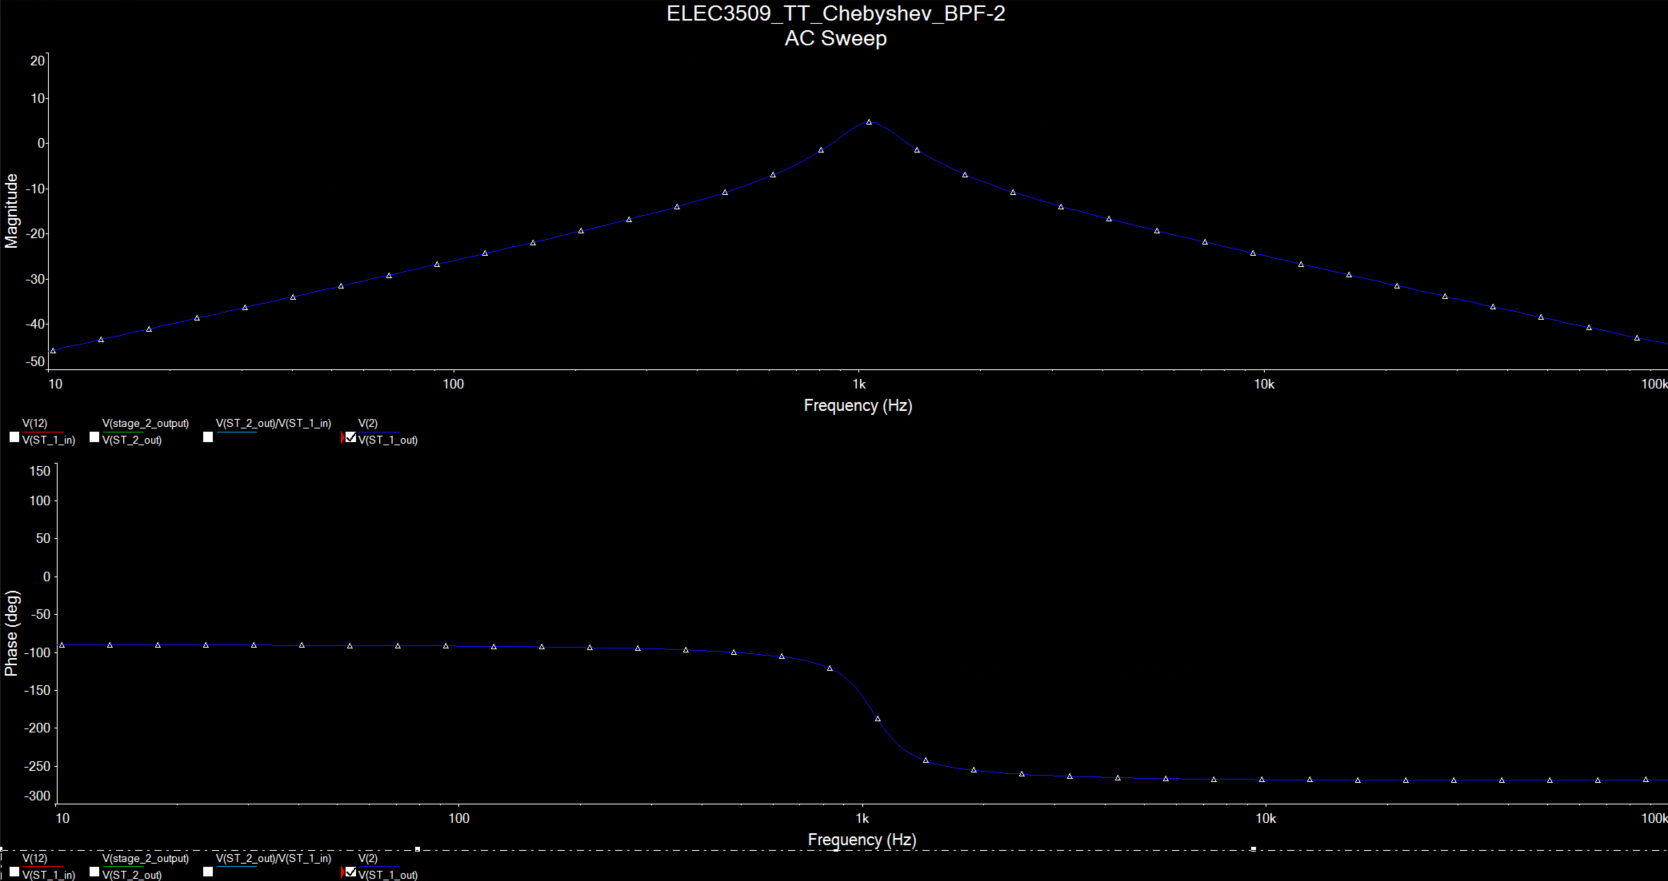
\includegraphics[width=0.6\textheight]{stageA_gain_stand.png}
		\captionof{figure}{Simulated Response Plot, Using Standard Components Values, of The $H_A(S)$ Filter Circuit}
		\label{f:stageA_gain_stand}
	\end{figure}	
	\begin{figure}[htbp]
		\centering
		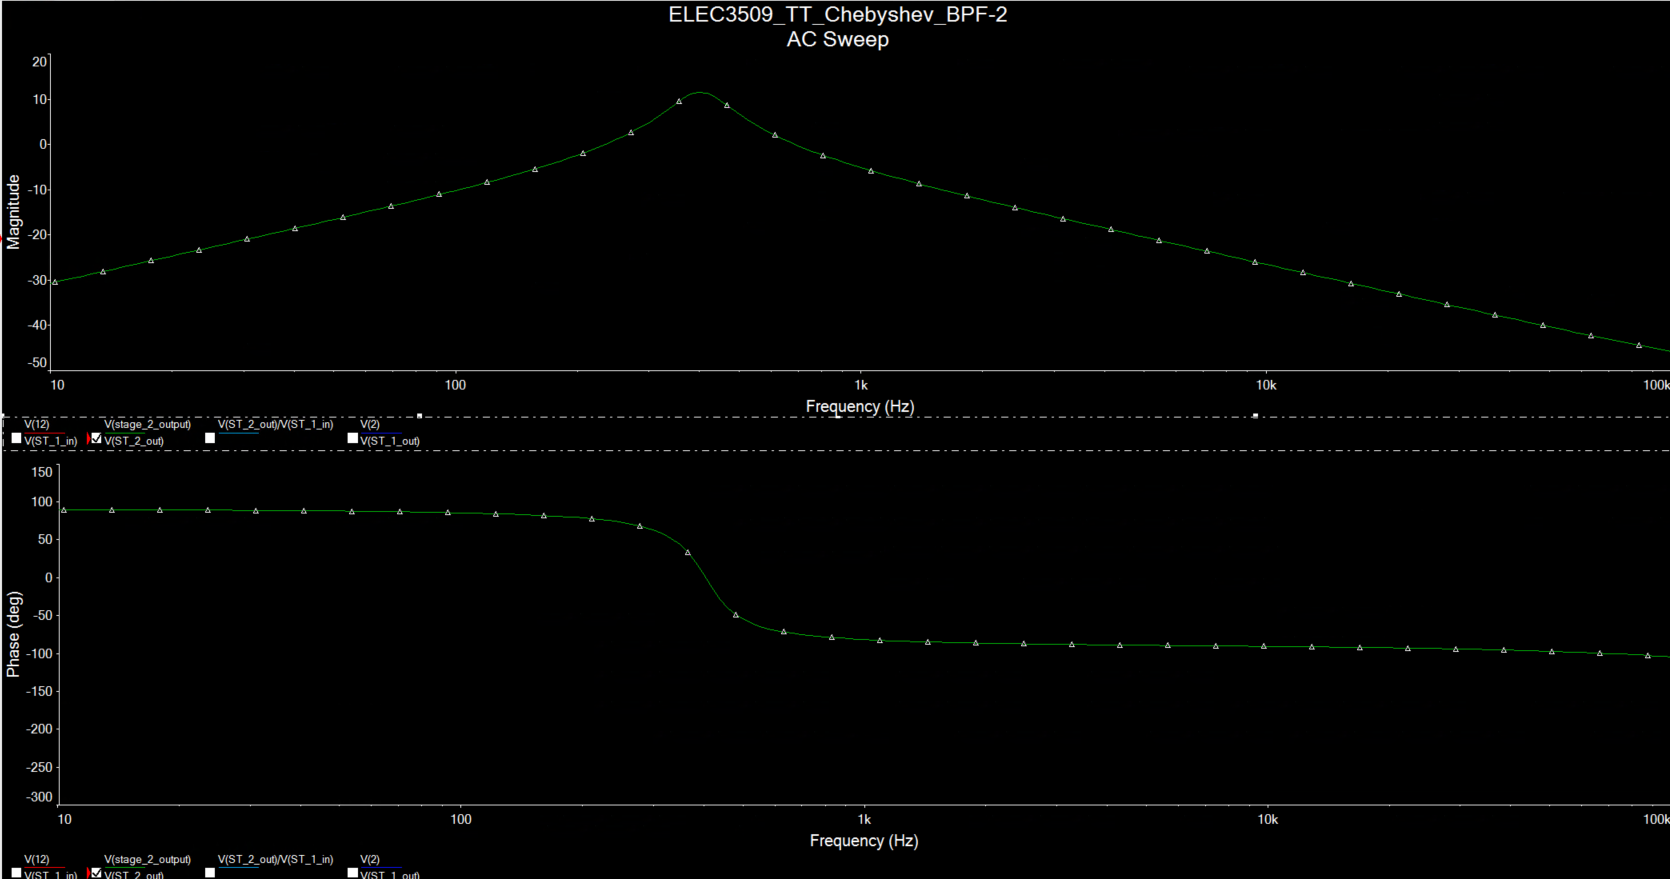
\includegraphics[width=0.6\textheight]{stageB_gain_stand.png}
		\captionof{figure}{Simulated Response Plot, Using Standard Components Values, of The $H_B(S)$ Filter Circuit}
		\label{f:stageB_gain_stand}
	\end{figure}	
	
	\noindent In comparison between Fig. \ref{f:stageA_gain_stand} and Fig. \ref{f:stageA_gain}, the gain in the simulated response plot using standard components values is a fairly close match to the simulated response plot for $H_A(S)$. 
	Likewise, the comparison between Fig. \ref{f:stageB_gain_stand} and Fig. \ref{f:stageB_gain} shows that the gain in the simulated response plot using standard components values is afairly close match to the simulated response plot for $H_B(S)$.

	\pagebreak
	\section{Verification}
	\begin{table}[htbp]
		\centering
		\captionof{table}{Summary Table for the \textcolor{green}{Overall Filter Circuit}}
		\begin{tabular}{|c|c|c|c|}
			\hline
			& Theoretical & Simulated & Simulated Standard Values\\
			\hline\hline
			$A_{mid}$ & \SI{-0.0259}{\decibel} & \SI{-0.0671}{\decibel} & \SI{-0.9671}{\decibel}\\
			\hline
			$f_{lower}$ & \SI{338.64}{\hertz} & \SI{339.7346}{\hertz} & \SI{371.72285}{\hertz}\\
			\hline
			$f_{upper}$ & \SI{1.0168}{k\hertz} & \SI{1.0139}{k\hertz} & \SI{1.1507}{k\hertz}\\
			\hline
			BW & \SI{4261}{\radian/\second} & \SI{4236}{\radian/\second} & \SI{4894}{\radian/\second}\\
			\hline
			Q & 0.8653 & 0.8706 & 0.8396\\
			\hline
			$\omega_o$ & \SI{3687}{\radian/\second} & \SI{3688}{\radian/\second} & \SI{4109}{\radian/\second}\\
			\hline 
		\end{tabular}
	\label{onlyTable}
	\end{table}
	\noindent As shown in Table \ref{onlyTable}, the gain of the theoretical values is \SI{-0.0259}{\decibel} which is very close to the gain of the simulated values is \SI{-0.0671}{\decibel}. 
	Also, the gain of the simulated standard values is \SI{-0.9671}{\decibel} which is very close to both theoretical and simulated gain.
	These results statisfy the design requirements of the Chebyshev filter project as it is within $\pm$\SI{1.0}{\decibel} gain error.
	Also, the gain results are within the trageted passband gain of +\SI{0.0}{\decibel} to \SI{-3.0}{\decibel} which what is desired for this project to achieve\\\\
	Table \ref{onlyTable} also shows that $f_{lower}$ of the theoretical values is \SI{338.64}{\hertz} while the $f_{lower}$ of the simulated values is \SI{339.7346}{\hertz}.
	The error percentage between the theoretical and simulated gain is 0.3\%.
	The $f_{lower}$ value of the simulated standard values is \SI{371.72285}{\hertz} which has a 9\% error percentage.
	These results do not satisfy the design requirements.
	Many attempts were done to reduce the 9\% to 8\% so that the $f_{lower}$ of the simulated standard values meet the specified requirements.
	Due to the fact that the closest resistance and capactiance values were used, and that the calculations were student number based, the error percentage in the $f_{lower}$ of the simulated standard values could not be further reduced while maintaining the other design requirements.
	An extra 1\% error would not have a huge impact on the design and therefore, the number was recorded and reported.\\\\
	Similarly, the same problem was encounter when measureing $f_{upper}$.
	Table \ref{onlyTable} also shows that $f_{upper}$ of the theoretical values is \SI{1.0168}{k\hertz} while the $f_{upper}$ of the simulated values is \SI{1.0139}{k\hertz}.
	The error percentage between the theoretical and simulated gain is approximately 0.3\%
	The $f_{upper}$ value of the simulated standard values is\SI{1.1507}{k\hertz} which has a 13\% error percentage.	
	These results do not satisfy the design requirements.
	Many attempts were done to reduce the 13\% to 8\% so that the $f_{upper}$ of the simulated standard values meet the specified requirements.	
	Due to the fact that the closest resistance and capactiance values were used, and that the calculations were student number based, the error percentage in the $f_{upper}$ of the simulated standard values could not be further reduced while maintaing the other design requirements.\\\\
	The ripple was measured and found to be approximately \SI{3}{\decibel} for both peaks of the gain plot for the simulated and standrad simulated values filter as shown in Fig. \ref{f:simulated_ripple} and Fig. \ref{f:simulated_ripple1}\\\\
	Table \ref{onlyTable} also shows a bandwidth of \SI{4261}{\radian/\second} for the theoretical values while the simulated bandwidth value is  \SI{4236}{\radian/\second}.
	These results are almost identical and shows a very low error percentage which indicates that the simulated filter using theoretical values satifies the design requirements of this project.
	On the other side, the bandwidth of the simulated standard values is \SI{4894}{\radian/\second} which is slighly larger than the theoretical and simulated values.\\\\
	The quality factor, Q, of the theoretical, simulated, and standard simulated values are fairly close to each other. 
	The Q values are 0.8653, 0.8706, and 0.8396 respectively.\\\\
	Table \ref{onlyTable} also shows that $\omega_o$ of the theoretical values is \SI{3687}{\radian/\second} while the $\omega_o$ of the simulated values is \SI{3688}{\radian/\second} which has a very small error percentage in comparison $\omega_o$ value of the theoretical value.
	The $\omega_o$ value of the simulated standard values is \SI{4109}{\radian/\second} which slighly larger than desired.\\\\
	6 Op-Amps total were used and they were all type TL082.\\
	The supply voltages to the circuit were \SI{+15}{\volt}.\\
	The output voltage swing is greater than $\pm$\SI{10}{\volt} which was verified through the simulation.
	
	\section{Discussion}
	Chebyshev filters can be analog or digital filters.
	In this lab, an analog Chebyshev filter was constructed and simulated.
	Chebyshev filters have a steeper roll-off tha other filters such as Butterworth filter and they have passband ripple or stopband ripple.
	As shown in different gain plots of the various filters built in this lab, the gain plot has a passband ripple of \SI{3}{\decibel} as the first peak is approached and a passband ripple of \SI{3}{\decibel} as the second peak is approached.\\\\
	Due to the passband ripple shonw in the multiple gain plots, teh filter has a much smoother reponse.
	The filters built in this lab are $4^{th}$ order filters.
	The order of a Chebyshev filter is equal to the number of reactive components.
	In our case, the filter circuit has four reactive components which are the four capacitors used to construct the circuit.\\\\
	For the phase of the overall filter circuit, it is seen that the phase starts droping below \SI{0}{degrees} when $f_{lower}$ is approached.
	The phase starts dropping and continues to drop to \SI{-360}{degrees} and then becomes constat at \SI{-360}{degrees} when $f_{upper}$ is approached.
	
	\pagebreak
	\section{Conclusion}
	By the end of this laboratory, a fourth-order bandpass filter was designed and simulated based on theoretical components values.
	Then, another a fourth-order bandpass filter was constructed and simulated using standard components values.
	The purpose was to provide the junior analog designer an experience with second-order circuits as well as the Chebyshev filter response in the context of a design problem [1].\\\\
	In day 1, a fourth-order bandpass filter was simulated using the theoretical values done in the prelab.
	The desing was simulated and verified and data were collected.
	The gain of the theoretical values is \SI{-0.0259}{\decibel} which is very close to the gain of the simulated values is \SI{-0.0671}{\decibel}.
	$f_{lower}$ of the theoretical values is \SI{338.64}{\hertz} while the $f_{lower}$ of the simulated values is \SI{339.7346}{\hertz}.
	$f_{upper}$ of the theoretical values is \SI{1.0168}{k\hertz} while the $f_{upper}$ of the simulated values is \SI{1.0139}{k\hertz}.\\\\
	In day 2, a fourth-order bandpass filter was simulated using the standard compnents values.
	The desing was simulated and verified and data were collected.
	The gain of the standard simulated values is \SI{-0.9671}{\decibel} which is fairly close to the gain of the theoretical and simulated values.
	$f_{lower}$ of the standard simulated values is \SI{371.72285}{\hertz} while $f_{upper}$ of the standard simulated values is \SI{1.1507}{k\hertz}.
	These results did not satisfy the $\pm$8\% error range. 
	However, the error percentage was close enough that a decision of recording and reporting these data was made.\\\\
	All the other requirments for both the simulated and standard simulated values were meet as stated in the design project requirements.
	
	\pagebreak
	\section{References}
	[1] “Lab 4: Active Band-Pass Filter Project,” Carleton Univeristy, Ottawa, 2017.
	
	\pagebreak
	\section{Appendix}
		\begin{figure}[htbp]
		\centering
		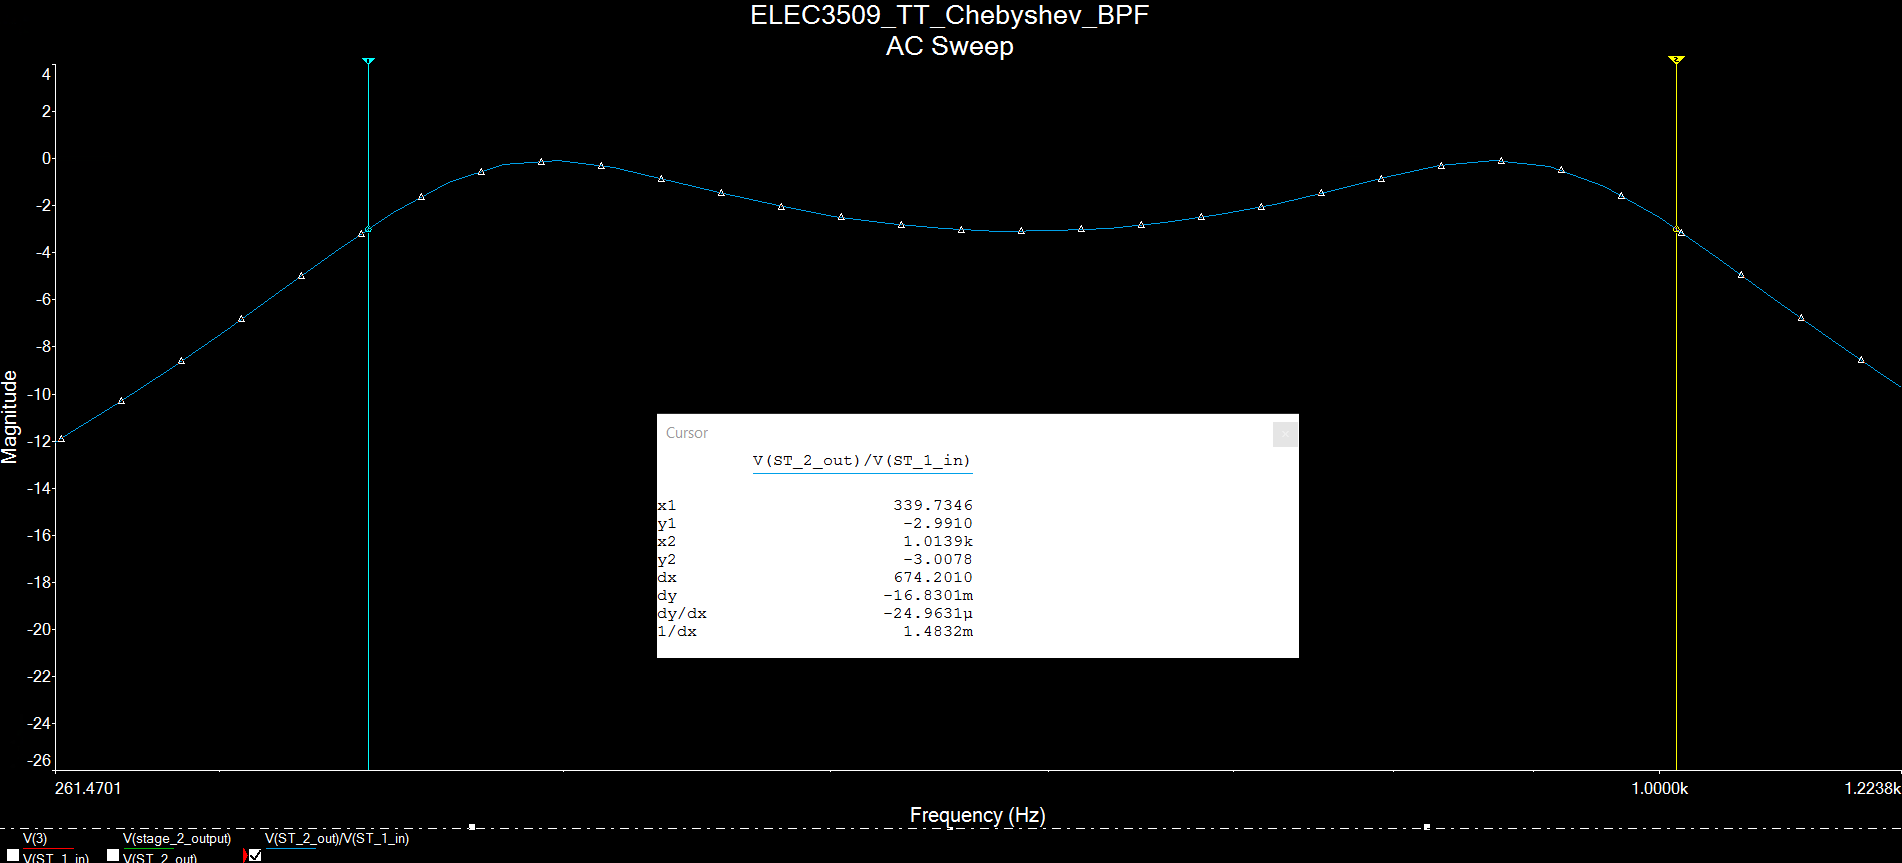
\includegraphics[width=0.6\textheight]{measured_simulated.png}
		\captionof{figure}{Simulated Response Plot of The Overall Filter Circuit}
		\label{f:measured_simulated}
	\end{figure}
	
	\begin{figure}[htbp]
		\centering
		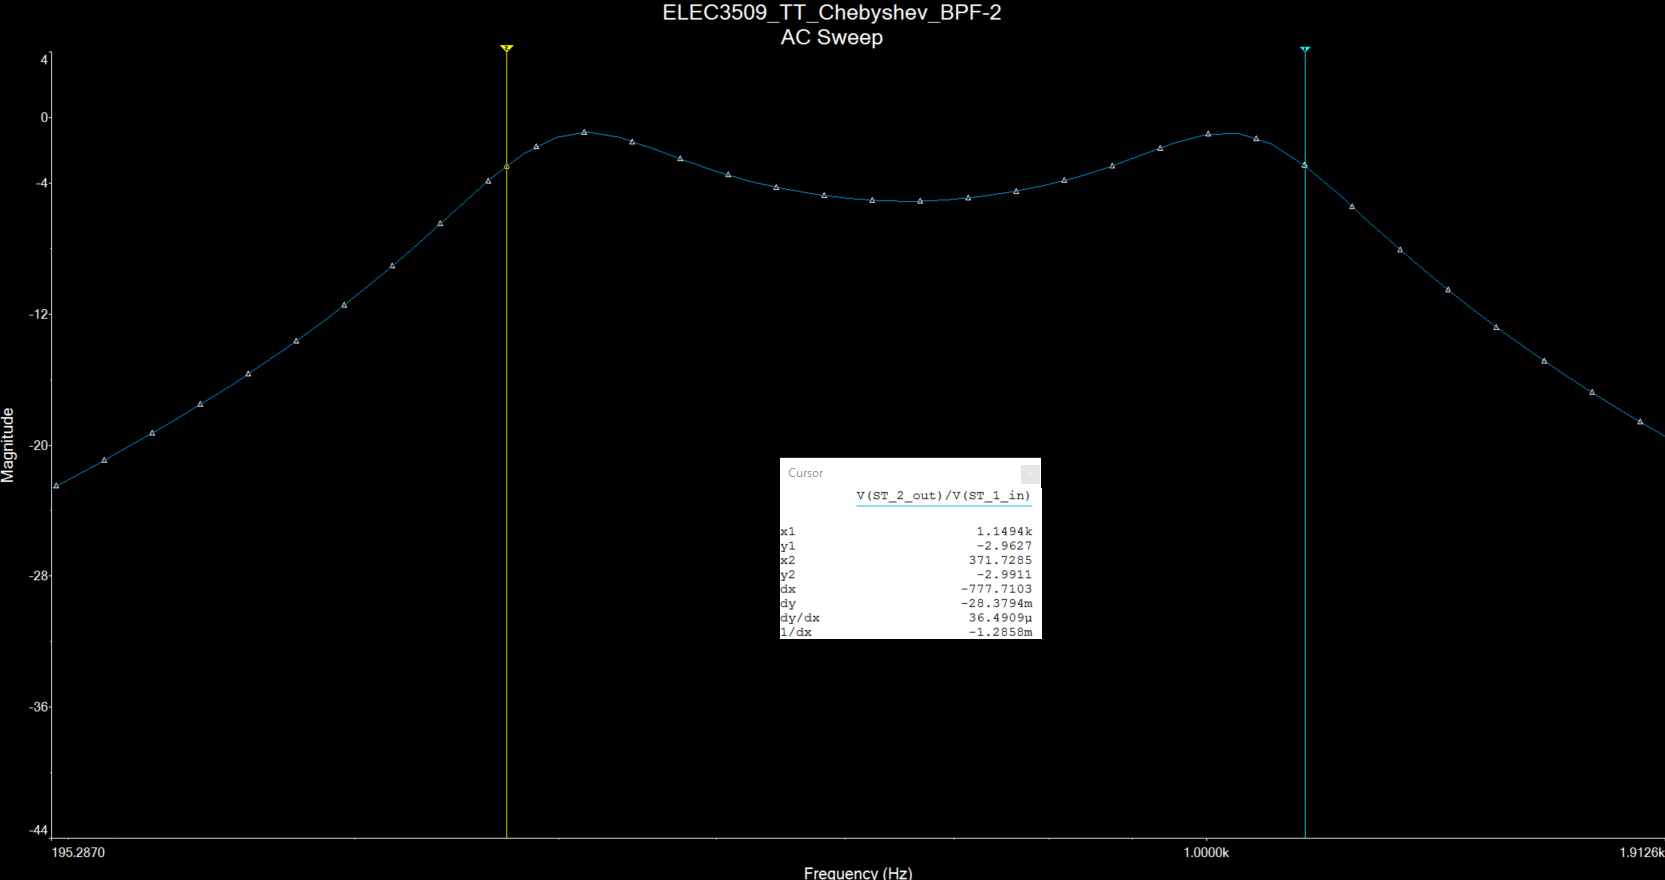
\includegraphics[width=0.6\textheight]{measured_standSimulated.png}
		\captionof{figure}{Standard Simulated Response Plot of The Overall Filter Circuit}
		\label{f:measured_standSimulated}
	\end{figure}

	\pagebreak
	
	\begin{figure}[htbp]
		\centering
		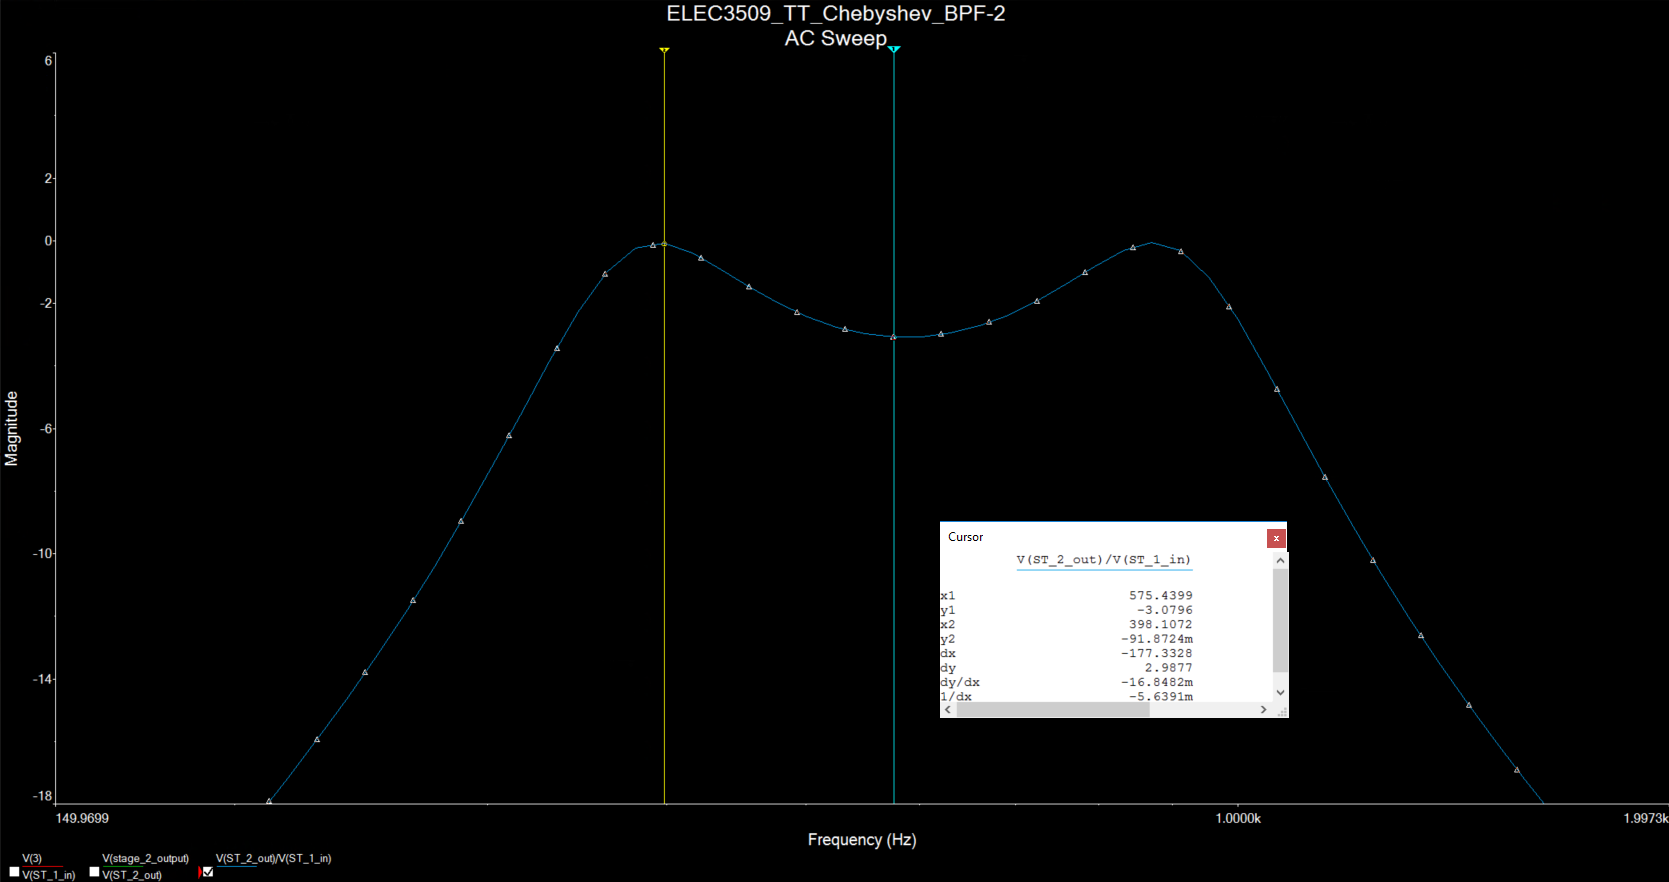
\includegraphics[width=0.6\textheight]{simulated_ripple.png}
		\captionof{figure}{Simulated Ripple 1}
		\label{f:simulated_ripple}
	\end{figure}

	\begin{figure}[htbp]
		\centering
		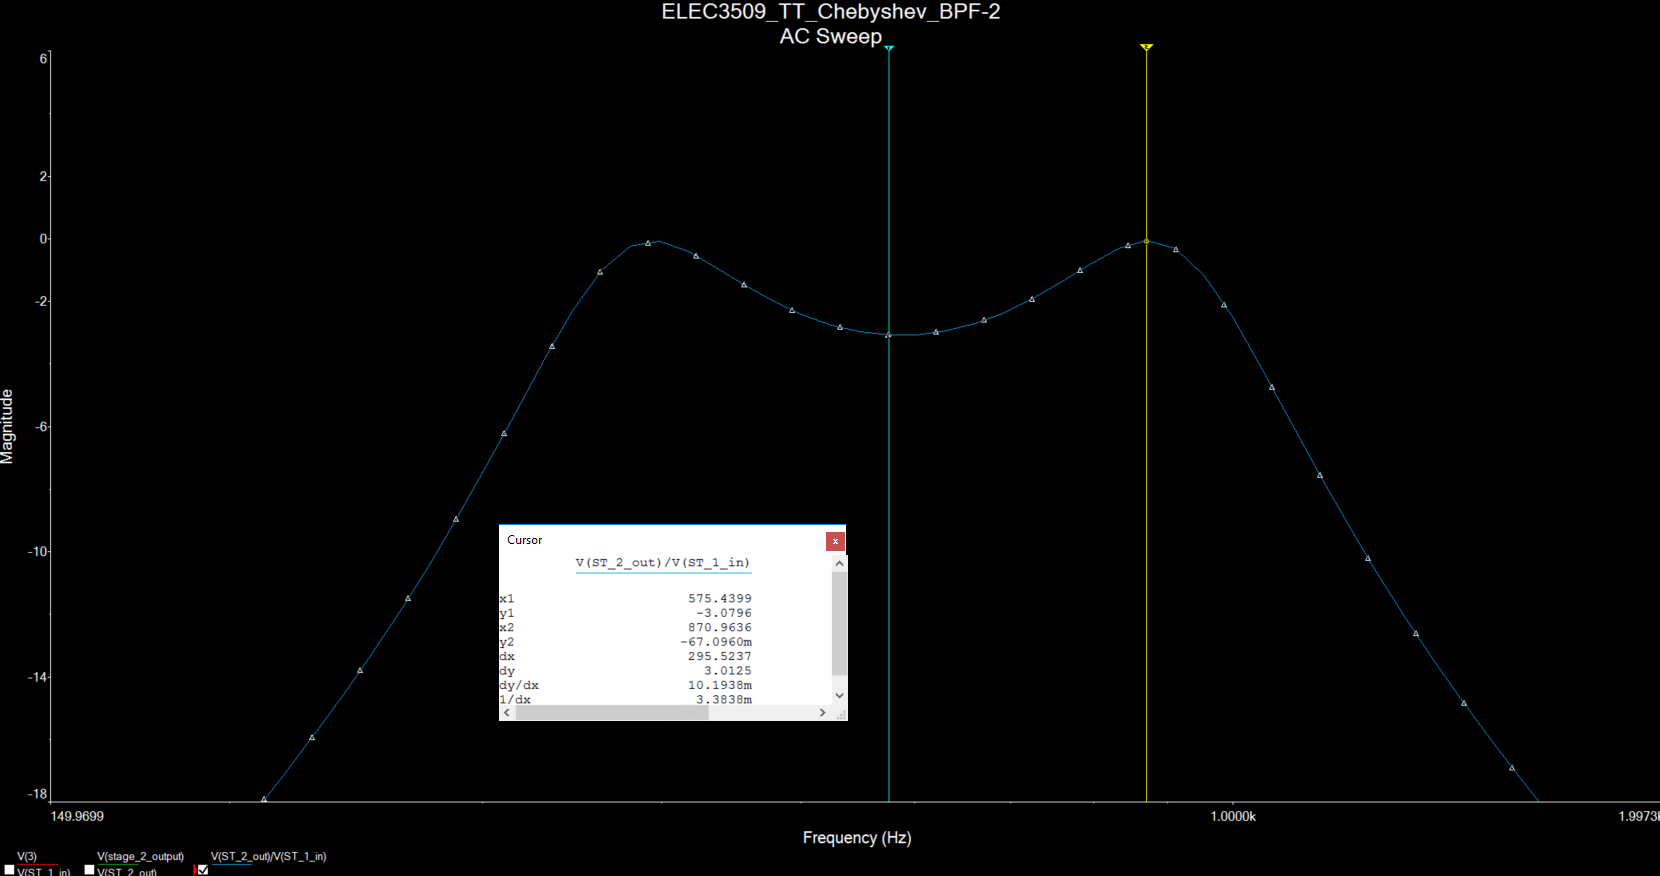
\includegraphics[width=0.6\textheight]{simulated_ripple1.png}
		\captionof{figure}{Standard Simulated Ripple}
		\label{f:simulated_ripple1}
	\end{figure}
	%%%%%% MATLAB CODE %%%%%%
	
	%clc
	
	%///////////////////// CALCULATED FILTER VALUES ///////////////////////////
	
	%Calculating A and B from student number
	%X = 101078550
	%B = mod(X,1033)
	%A = mod(X,1031)
	
	%Upper and lower frequency
	%f1 = [(A^5)/(5.534*10^9)]-[(A^4)/(2.11*10^6)]+[(A^3)/(2287)]-[(A^2)/(6.1)]+[20.2*A]+[750]
	%sigma = -((B^2)/180000)+(B/173)+0.5
	%fh = f1*(1+sigma)
	
	%Upper and lower cut-off angular frequency
	%wlow = 2*pi*f1
	%whigh = 2*pi*fh
	
	%Bandwidth of overall filter
	%Bw = 2*pi*(fh-f1)
	
	%Corner frequency of the filter
	%wo = 2*pi*(sqrt(fh*f1))
	
	%Q value for the overall filter
	%Q = wo/Bw
	
	%///////////////////// TEST FILTER SPECIFICATIONS /////////////////////////
	
	%Test filter specifications
	%a = 0.7079^2;
	%b = 0.6449;
	%c = 0.7079;
	%NumX = a*(Bw^2)
	%Dem1 = b*Bw;
	%Dem2 = 2*(wo^2)+c*(Bw^2);
	%Dem3 = b*Bw*(wo^2);
	%Dem4 = wo^4;
	%Num1 = sqrt(NumX)
	%Num2 = sqrt(NumX)
	
	%%%SPECIAL MATLAB MAJIC. TOTALLY ORIGINAL%%%
	%Factoring the expanded polynomial to get two TF for Stage 1 and Stage 2
	%polyCoeff = [1 Dem1 Dem2 Dem3 Dem4];
	%polyRoots = roots(polyCoeff);
	%poly1Coeff = poly(polyRoots(1:2));
	%poly2Coeff = poly(polyRoots(3:4));
	
	
	%Corner frequencies for Stage 1 and Stage 2
	%w01 = sqrt(poly1Coeff(3))
	%w02 = sqrt(poly2Coeff(3))
	
	
	%Q values for Stage 1 and Stage 2
	%Q1 = w01/(poly1Coeff(2))
	%Q2 = w02/(poly2Coeff(2))
	
	%Bandwidth values for Stage 1 and Stage 2
	%Bw1 = poly1Coeff(2)
	%Bw2 = poly2Coeff(2)
	
	
	%Capacitors (Chosen from the capacitors given)
	%C1 = 22e-9;
	%C2 = 33e-9;
	
	%R for both stage one and two of the filter
	%R1 = 1/(w01*C1)
	%R2 = 1/(w02*C2)
	
	%Rq for both stage one and two of the filter
	%Rq1 = R1*Q1
	%Rq2 = R2*Q2
	%r = 9500
	
	%Rin for both stage one and stage two of the
	%R31 = r/(R1*C1*(Num1))
	%R32 = r/(R2*C2*(Num2))
	
	%%%MORE SPECIAL MATLAB MAJIC. TOTALLY ORIGINAL%%%
	%Num = [NumX 0 0] ;
	%Dem = [1 Dem1 Dem2 Dem3 Dem4];
	
	%Frequency range and the value of s
	%f = 100:50:1e4;
	%s = 2*pi*f*j;
	
	%Magnitude of the frequency response in dB
	%FR1 = 20*log10(abs(polyval(Num,s) ./ polyval(Dem,s)));
	%figure(1)
	%semilogx(f,FR1)
	%grid on;
	%gainMax = max(FR1)
	%xlabel ('Frequency (Hz)')
	%ylabel ('Magnitude (dB)')
	%axis ([0 1e4 -90 10])
	%format short e
	
	%%EVEN MORE SPECIAL MATLAB MAJIC. TOTALLY ORIGINAL%%%
	% FIRST STAGE PLOT
	
	
	%NumS1 = [Num1 0];
	%DemS1 = [poly1Coeff(1) poly1Coeff(2) poly1Coeff(3)];
	
	%Frequency range and the value of s
	%f = 100:50:1e4;
	%s = 2*pi*f*j;
	
	%Magnitude of the frequency response in dB
	%FR2 = 20*log10(abs(polyval(NumS1,s) ./ polyval(DemS1,s)));
	%figure(2)
	%semilogx(f,FR2)
	%grid on;
	%gainMax1 = max(FR2)
	%xlabel ('Frequency (Hz)')
	%ylabel ('Magnitude (dB)')
	%axis ([0 1e4 -90 10])
	
	
	% SECOND STAGE PLOT
	
	%NumS2 = [Num2 0];
	%DemS2 = [poly2Coeff(1) poly2Coeff(2) poly2Coeff(3)];
	
	%Frequency range and the value of s
	%f = 100:50:1e4;
	%s = 2*pi*f*j;
	
	%Magnitude of the frequency response in dB
	%FR3 = 20*log10(abs(polyval(NumS2,s) ./ polyval(DemS2,s)));
	%figure(3)
	%semilogx(f,FR3)
	%grid on;
	%gainMax2 = max(FR3)
	%xlabel ('Frequency (Hz)')
	%ylabel ('Magnitude (dB)')
	%axis ([0 1e4 -90 20])
\end{document}